\documentclass[11pt,a4paper]{article}
%-------------------------------------------
%---Packages--------------------------------
%-------------------------------------------
\usepackage[utf8]{inputenc}
%\usepackage[T1]{fontenc}
%\usepackage{txfonts}
\usepackage{amsmath}
\usepackage{amsthm}
\usepackage{amsfonts}
\usepackage{array}
\usepackage{amssymb}
\usepackage{blindtext}
\usepackage{caption}
\usepackage{color}
\usepackage{csquotes}	    %
\usepackage{enumitem}	    %pour mieux bosser avec les listes. ajoute option label
\usepackage[yyyymmdd]{datetime}        %pour définir date custom
\usepackage{etaremune}
\usepackage{environ}
\usepackage{fancybox}
\usepackage{fancyhdr} 	    % Custom headers and footers
\usepackage{fancyref}
%\usepackage{float}
\usepackage{floatrow}       %float and floatrow can't be together...
\usepackage{gensymb}
\usepackage{graphicx}
\usepackage[colorlinks=true, linkcolor=purple, citecolor=cyan]{hyperref}
\usepackage{footnotebackref}
\usepackage{lipsum}
\usepackage{mathtools}
\usepackage{multicol}	    %gérer plusieurs colonnes
\usepackage{setspace}
\usepackage{subcaption}
\usepackage{todonotes}	    %Bonne gestion des TODOs
%TODO commenté pour tester l'utilité... à voir% \usepackage[tc]{titlepic}      %Permet de mettre une image en page de garde
\usepackage{tikz}	    % Pour outil de dessin puissant
\usepackage{ulem}	    %underline sur plusieurs lignes (avec \uline{})
\usepackage{vmargin} 	    %gestion des marges, avec dans l'ordre : gauche, haut, droit, bas, en-tête, entre en-tête et texte, bas de page, hauteur entre bas de page et texte
\usepackage{wrapfig}
\usepackage{xcolor}
\usepackage{xparse}                    %Pour utiliser NewDocumentCommand et des arguments 'mmooo'
%\usepackage{fullpage} 	    %supprime toutes les marges allouées aux notes, aussi en haut et en bas

%\ExplSyntaxOn
\pagestyle{fancyplain}	    %Makes all pages in the document conform to the custom headers and footers

%-------------------------------------------
%---Document Commands-----------------------
%---------------------------{----------------
\NewDocumentCommand{\framecolorbox}{oommm}
 {% #1 = width (optional)
  % #2 = inner alignment (optional)
  % #3 = frame color
  % #4 = background color
  % #5 = text
  \IfValueTF{#1}%
   {\IfValueTF{#2}%
    {\fcolorbox{#3}{#4}{\makebox[#1][#2]{#5}}}%
    {\fcolorbox{#3}{#4}{\makebox[#1]{#5}}}%
   }%
   {\fcolorbox{#3}{#4}{#5}}%
 }%
%------------------------------------------------
%------------------ENGLISH----------------------
%----------------------------------------------

\NewDocumentCommand{\epflTitle}{mO{Olivier Cloux}O{\today}O{Notes de Cours en}D<>{../../Common}}%Arguments : Matière, Auteur, Date, Titre du doc
{
\begin{titlepage}
    \vspace*{\fill}
    \begin{center}
        \normalfont \normalsize
        \textsc{Ecole Polytechnique Fédérale de Lausanne} \\ [25pt] % Your university, school and/or department name(s)
        \textsc{#4} %Titre du doc
        \\ [0.4 pt]
        \horrule{0.5pt} \\[0.4cm] % Thin top horizontal rule
        \huge #1 \\ % Matière
        \horrule{2pt} \\[0.5cm] % Thick bottom horizontal rule
        
\includegraphics[width=8cm]{#5/EPFL_logo}
        ~\\[0.5 cm]
        \small\textsc{#2}\\[0.4cm]
        \small\textsc{#3}\\
        ~\\
        ~\\
        
\includegraphics[scale=0.5]{#5/creativeCommons}
    \end{center}
    \vspace*{\fill}
\end{titlepage}
}


%-------------------------------------------
%-------------MATH NEW COMMANDS-------------
%-------------------------------------------
\newcommand{\somme}[2]{\ensuremath{\sum\limits_{#2}^{#1}}}
\newcommand{\produit}[2]{\ensuremath{\prod\limits_{#2}^{#1}}}
\newcommand{\limite}{\lim\limits_}
\newcommand{\llimite}[3]{\limite{\substack{#1 \\ #2}}\left(#3\right)}	%limites à deux condiitons
\newcommand{\et}{\mbox{ et }}
\newcommand{\deriv}[1]{\ensuremath{\, \mathrm d #1}}	%sigle dx, dt,dy... des dérivées/intégrales
%\newcommand{\fx}{\ensuremath{f'(\textbf{x}_0 + h}}
\newcommand{\ninf}{\ensuremath{n \to \infty}}	       %pour les limites : n tend vers l'infini
\newcommand{\xinf}{\ensuremath{x \to \infty}}	       %pour les limites : x tend vers l'infini
\newcommand{\infint}{\ensuremath{\int_{-\infty}^{\infty}}}
\newcommand{\xo}{\ensuremath{x \to 0}}									%x to 0
\newcommand{\no}{\ensuremath{n \to 0}}									%n zéro
\newcommand{\xx}{\ensuremath{x \to x}}									%x to x
\newcommand{\Xo}{\ensuremath{x_0}}										%x zéro
\newcommand{\X}{\ensuremath{\mathbf{X}} }
\newcommand{\A}{\ensuremath{\mathbf{A}} }
\newcommand{\R}{\ensuremath{\mathbb{R}} }								%ensemble de R
\newcommand{\rn}{\ensuremath{\mathbb{R}^n} } 							%ensemble de R de taille n
\newcommand{\Rm}{\ensuremath{\mathbb{R}^m} }  							%ensemble de R de taille m
\newcommand{\C}{\ensuremath{\mathbb{C}} }
\newcommand{\N}{\ensuremath{\mathbb{N}} }
\newcommand{\Z}{\ensuremath{\mathbb{Z}} }
\newcommand{\Q}{\ensuremath{\mathbb{Q}} }
\newcommand{\rtor}{\ensuremath{\R \to \R} }
\newcommand{\pour}{\mbox{ pour }}
\newcommand{\coss}[1]{\ensuremath{\cos\(#1\)}}						%cosinus avec des parenthèses de bonne taille (genre frac)
\newcommand{\sinn}[1]{\ensuremath{\sin\(#1\)}}					%sinus avec des parentèses de bonne taille (genre frac)
\newcommand{\txtfrac}[2]{\ensuremath{\frac{\text{#1}}{\text{#2}}}}		%Fractions composées de texte
\newcommand{\evalfrac}[3]{\ensuremath{\left.\frac{#1}{#2}\right|_{#3}}}
\renewcommand{\(}{\left(}												%Parenthèse gauche de taille adaptive
\renewcommand{\)}{\right)}
\newcommand{\longeq}{=\joinrel=}												%Parenthèse droite de taille adaptive


%-------------------------------------------------------
%------------------MISC NEW COMMANDS--------------------
%-------------------------------------------------------
\newcommand{\degre}{\ensuremath{^\circ}}
%\newdateformat{\eudate}{\THEYEAR-\twodigit{\THEMONTH}-\twodigit{\THEDAY}}



%-------------------------------------------------------
%------------------TEXT NEW COMMANDS--------------------
%-------------------------------------------------------
\newcommand{\ts}{\textsuperscript}
\newcommand{\evid}[1]{\textbf{\uline{#1}}}        %mise en évidence (gras + souligné)



%\newcommand{\Exemple}{\underline{Exemple}}
\newcommand{\Theoreme}{\underline{Théorème}}
\newcommand{\Remarque}{\underline{Remarque}}
\newcommand{\Definition}{\underline{Définition} }
\newcommand{\skinf}{\sum^{\infty}_{k=0}}
\newcommand{\combi}[2]{\ensuremath{\begin{pmatrix} #1 \\ #2 \end{pmatrix}}}	%combinaison parmi 1 de 2
\newcommand{\intx}[3]{\ensuremath{\int_{#1}^{#2} #3 \deriv{x}}}				%intégrale dx
\newcommand{\intt}[3]{\ensuremath{\int_{#1}^{#2} #3 \deriv{t}}}				%intégrale dy
\newcommand{\misenforme}{\begin{center} Mis en forme jusqu'ici\\ \line(1,0){400}\\ normalement juste, mais à améliorer depuis ici\end{center}}	%raccourci pour mise en forme
\newcommand*\circled[1]{\tikz[baseline=(char.base)]{
            \node[shape=circle,draw,inner sep=1pt] (char) {#1};}}			%pour entourer un chiffre
\newcommand{\horrule}[1]{\rule{\linewidth}{#1}} 				% Create horizontal rule command with 1 argument of height

\theoremstyle{definition}
\newtheorem{exemp}{Exemple}
\newtheorem{examp}{Example}


%-------------------------------------------
%---Environments----------------------------
%-------------------------------------------
\NewEnviron{boite}[1][0.9]{%
	\begin{center}
		\framecolorbox{red}{white}{%
			\begin{minipage}{#1\textwidth}
 	 			\BODY
			\end{minipage}
		}
	\end{center}
}
\NewEnviron{blackbox}[1][0.9]{%
	\begin{center}
		\framecolorbox{black}{white}{%
			\begin{minipage}{#1\textwidth}
 	 			\BODY
			\end{minipage}
		}
	\end{center}
}
\NewEnviron{exemple}[1][0.8]{%
    \begin{center}
        \framecolorbox{white}{gray!20}{%
            \begin{minipage}{#1\textwidth}
                \begin{exemp}
                    \BODY
                \end{exemp}
            \end{minipage}
        }
    \end{center}
}
\NewEnviron{suiteExemple}[1][0.8]{%
    \begin{center}
        \framecolorbox{white}{gray!20}{%
            \begin{minipage}{#1\textwidth}
                \BODY
            \end{minipage}
        }
    \end{center}
}
\NewEnviron{colExemple}[1][0.8]{%
    \begin{center}
        \framecolorbox{white}{gray!20}{%
            \begin{minipage}{#1\columnwidth}
                \begin{exemp}
                    \BODY
                \end{exemp}
            \end{minipage}
        }
    \end{center}
}
\NewEnviron{example}[1][0.8]{%
    \begin{center}
        \framecolorbox{white}{gray!20}{%
            \begin{minipage}{#1\textwidth}
                \begin{examp}
                    \BODY
                \end{examp}
            \end{minipage}
	}
    \end{center}
}
\NewEnviron{systeq}[1][l]{
			\begin{center}
				$\left\{\begin{array}{#1}
					\BODY
				\end{array}\right.$
			\end{center}
 }





%-------------------------------------------
%---General settings-----------------------
%-------------------------------------------
\renewcommand{\headrulewidth}{1pt}										%ligne au haut de chaque page
\renewcommand{\footrulewidth}{1pt}										%ligne au pied de chaque page
\setstretch{1.6}
\author{Olivier Cloux}

\renewcommand{\contentsname}{Table des Matières}
\usepackage{fixme}
\usepackage{rotating}
%\usepackage{pdflscape}
\newcommand{\indep}{\perp\!\!\!\perp}
%%%%%%%%%%%%%%%%%%%%%%%%%%%%%%%%%%%%%%%%%%%%
%%TODO : Supprimer quand plus de todo %%%%%%
\marginparwidth = 75pt
\textwidth = 400pt
%%%%%%%%%%%%%%%%%%%%%%%%%%%%%%%%%%%%%%%%%%%%

\usepackage{titlesec}
\titleformat{\section}{\center\Large\bfseries}{}{0pt}{Module \thesection:\ }
\numberwithin{equation}{section}

\begin{document}
\setstretch{1}
\epflTitle{Modèles Stochastiques}[Olivier Cloux][Automne 2017]
%\begin{multicols}{2}
	\tableofcontents
%\end{multicols}
\newpage
\section{Variables Aléatoires}
\subsection{Bases de proba}
\subsubsection{Axiomes de probabilités}
$\zeta_i$ le résultat de la \textit{i-ème} expérience. $A = \{\zeta_1,\zeta_2,\zeta_{17}\}$ un événement et $\Omega$ l'événement certain ($\emptyset$ l'événement impossible). L'espace de probabilité tel que nous le notons est 
\[\(\Omega, P(\cdot)\)\]
\begin{exemple}
	$\Omega$ peut être l'ensemble des résultats d'un jeter de dé, donc $\Omega = \{1,2,3,4,5,6\}$
\end{exemple}
Il en résulte les axiomes des probabilités : 
\begin{itemize}
	\item $P(A) \geq 0$
	\item $P(\Omega) = 1$
	\item DAns le cas où $\Omega$ est un ensemble \textit{fini}, si $A \cap B = \emptyset$ alors $P(A\cup B) = P(A) + P(B)$
	\item Dans le cas où $\Omega$ est un ensemble \textit{infini}, si $A_1,A_2,...$ est une suite d'événements telle que $A_i \cap A_j = \emptyset\ \forall i\neq j$ alors $P(\bigcup\limits{i=1}^{\infty} A_i) = \somme{\infty}{i=1}P(A_i)$
\end{itemize}
Et de ceci en suivent les corollaires : 
\begin{itemize}
	\item $P(\overline{A})  1 - P(A)$ où $\overline{A} = \Omega \backslash A$ 
	\item $P(A) \leq 1$
	\item $P(\emptyset) =0$
	\item $P(A \cup B) = P(A) + P(B) - P(A\cap B)$
	\item Si $A \subseteq B$ alors $P(A) \leq P(B)$
\end{itemize}
\subsubsection{Probabilité conditionnelle}
\[P(A|B) = \frac{P(A \cap B)}{P(B)}\]
\begin{boite}
	\evid{Théorème des probabilités totales :}
	Soit $\{A_1,A_2,...A_n\}$ une partition de $\Omega$ (donc $A_1 \cup A_2 \cup ... \cup A_n = \Omega$ et $A_i \cap A_j = \emptyset\ \forall i\neq j$). Alors 
	\begin{equation}
		\begin{array}{ll}
	P(B) &= P(B\cap A_1) + P(B\cap A_2) + ... + P(B \cap A_n)\\ &= \somme{n}{i=1} P(B \cap A_i) = \somme{n}{i=1} P(B|A_i)P(A_i)
		\end{array}
	\end{equation}
\end{boite}
\begin{exemple}
	Soit $\Omega$ la météo, partitionnée par $A_1 =$ Soleil et $A_2 =$ Pluie. Nous cherchons la probabilité de venir en vélo. En sachant que P(soleil) = 0.7 et P(pluie) = 0.3, P(vélo\textbar soleil) = 0.8 et P(vélo\textbar pluie) = 0.3.\\
	Alors P(vélo) = P(vélo\textbar soleil)P(soleil) + P(vélo\textbar pluie)P(pluie)
\end{exemple}
\begin{boite}
	\evid{Règle de Bayes}
	Soit à nouveau $\{A_1,...,A_n\}$ une partition de $\Omega$. Alors 
	\begin{equation}
		P(A_i|B) = \frac{P(B|A_i)P(A_i)}{\somme{n}{j=1} P(B|A_j)P(A_j)}
	\end{equation}
\end{boite}
\subsubsection{Indépendance}
\begin{boite}[0.7]
	$A$ et $B$ sont \textbf{indépendants} si $P(A\cap B) = P(A)P(B)$
\end{boite}
\evid{Corollaire} : $P(A|B) = P(A)$ et $P(B|A) = P(B)$\\
De même, trois événement sont indépendants si non seulement $P(A\cap B) = P(A)P(B)$ (et pareil pour toute combinaison de A,B,C) mais également $P(A\cap B\cap C) = P(A)P(B)P(C)$

\subsection{Variable aléatoire}
Une variable aléatoire (ou \textbf{v.a.} est une fonction $X$ qui map à chaque résultat $\zeta$ un réel $X(\zeta))$.
\[X : \Omega \mapsto \R\]
\begin{figure}[H]
	\center
	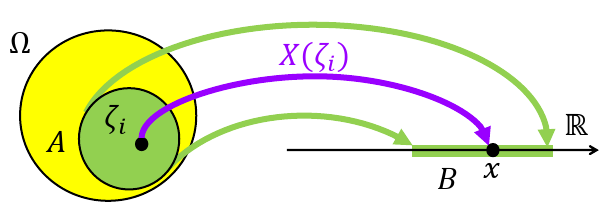
\includegraphics[scale=0.3]{images/variable_aleatoire}
	\caption{Représentation d'une variable aléatoire}
	\label{fig_variable_aleatoire}
\end{figure}
Comme visible à la figure \ref{fig_variable_aleatoire}, nous pouvons établir la bijection $B = \{X(\zeta) : \zeta \in A\}$ et $A = \{\zeta : X(\zeta) \in B\}$ avec évidemment $P(A) = P(B)$

\subsubsection{Fonction de répartition}
Toute v.a. est caractérisée par sa fonction de répartition (ou Cumulative Distribution Function, CDF) ; cette fonction représente la probabilité que $X$ prennent une valeur inférieure ou égale à un réel $x$ 
\begin{boite}
	\begin{equation}
		F_X(x) = P(X \leq x) = P(A)
	\end{equation}
\end{boite}
Cette fonction a plusieurs propriétés :
\begin{enumerate}[label=P\arabic*.]
	\item $0 \leq F_X(x) \leq 1$
	\item $\limite{x\to -\infty} F_X(x) = 0,\ \limite{x\to +\infty} F_X(x) = 1$
	\item $a < b \to F_X(a) \leq F_X(b)$
	\item $P(a < X \leq b) = F_X(b) - F_X(a)$
	\item $F_X(x)$ est continue à droite, i.e. $F_X(x) = \llimite{\epsilon \to 0}{\epsilon > 0}{F_X(x+\epsilon)} = F_X(x^+)$
\end{enumerate}
La variable aléatoire $X$ peut généralement prendre un ensemble de valeurs ; cet ensemble est appelé
 \textbf{le support} $S_X$, défini comme 
\begin{equation}
	S_X = \{X(\zeta)|\zeta \in \Omega\}
\end{equation}
Les valeurs que peut prend la variable aléatoire X peuvent être 
\begin{itemize}
	\item Discrètes (\ref{subfig_va_discrete}) : dénombrables (pas forcément fini). E.g. : des jets de dé. Alors $S_X=\{x_1,x_2,x_2,...\}$. Nous avons alors que $P(X=x_i) = F_X(x_i) - F_X(\overline{x_i})$
	\item Continues (\ref{subfig_va_continue}) : infini et indénombrable. E.g. : des mesures infiniment précises de température. Alors $P(X=x) = 0$\footnote{Bien que cela semble contre-intuitif, le nombre de valeurs est infini, donc chaque valeur exacte a une probabilité $\frac{1}{\infty}$ d'apparaître, soit nulle}
	\item Mixte (\ref{subfig_va_mixte}) : infini mais pas continu
\end{itemize}

\begin{figure}
	\center
	\begin{subfigure}{0.3\textwidth}
		\centering
		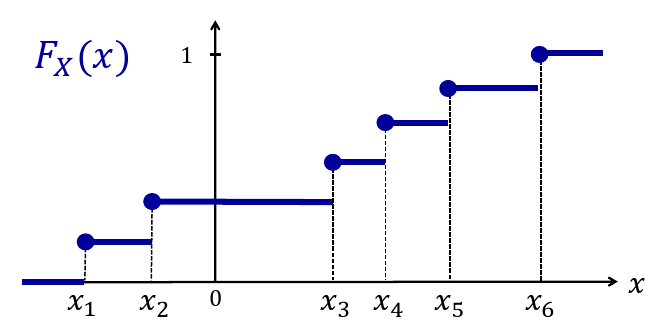
\includegraphics[scale=0.3]{images/va_discrete}
		\caption{v.a. discrète}
		\label{subfig_va_discrete}
	\end{subfigure}
		\begin{subfigure}{0.3\textwidth}
		\centering
		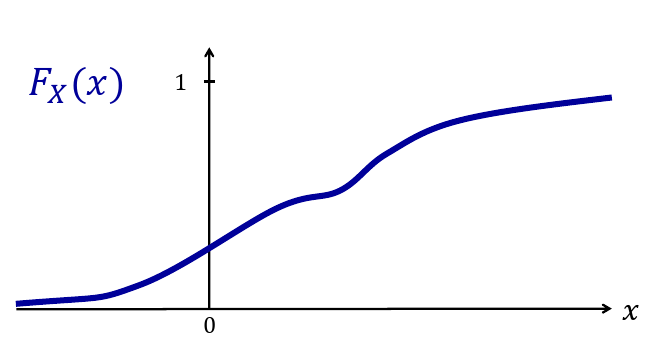
\includegraphics[scale=0.3]{images/va_continue}
		\caption{v.a. continue}
		\label{subfig_va_continue}
	\end{subfigure}
		\begin{subfigure}{0.3\textwidth}
		\centering
		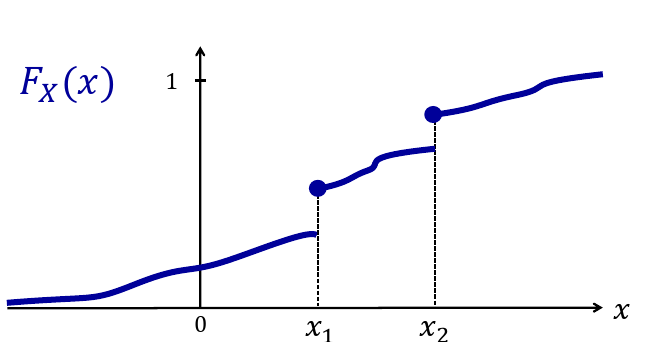
\includegraphics[scale=0.3]{images/va_mixte}
		\caption{v.a. mixte}
		\label{subfig_va_mixte}
	\end{subfigure}
	\caption{Différents types de support d'une variable aléatoire}
	\label{fig_type_support}
\end{figure}

\subsubsection{Densité de probabilité}
Aussi appelée Probability Density Function (PDF). Définie comme 
\begin{equation}
	f_X(x) = \frac{\deriv{F_X}}{\deriv{x}}(x)
	\label{eq_pdf}
\end{equation}
On distinguera des propriétés différentes si le support est discret ou continu. Dans le cas d'une v.a. \textbf{continue}, elles sont ainsi :
\begin{enumerate}[label=P\arabic*.]
	\item $f_x(x) \geq 0$
	\item $\infint f_X(x) \deriv{x} = F_X(\infty) - F_X(-\infty) = 1-0 = 1$
	\item $P(X\leq a) = F_X(a) = \int_{-\infty}^a f_X(x) \deriv{x}$
	\item $P(a < X \leq b) = F_X(b) - F_X(a) = \int_a^b f_X(x) \deriv{x}$, ce qui implique que $P(x < X \leq x+\Delta x) = f_X(x)\Delta x$ lorsque $\Delta x \to 0$
\end{enumerate}
Pour un support \textbf{discret}, nous utilisons les impulsions de Dirac $\delta(\cdot)$ afin de réécrire l'équation \ref{eq_pdf} comme 
\[f_X(x) = \somme{}{i}p_i\delta(x-x_i)\]
avec $p_i = P(X=x_i)$. Ceci donne lieu à des modifications des propriétés :
\begin{enumerate}[label=P\arabic*.]
	\item $p_i \geq 0$
	\item $\somme{}{i} p_i = 1$
	\item $P(X \leq a) = F_X(a) = \somme{}{x_i\leq a} p_i$
	\item $P(X = x_i) = F_X(x_i) - F_X(x_i^-) = p_i$
\end{enumerate}
\subsubsection{Fonction d'une variable aléatoire}
Prenons $g(\cdot)$ une fonction continue, et $X$ une v.a. continue. Alors 
\[Y = g(X)\] 
désigne aussi une v.a. continue\footnote{Pas en toute rigueur mathématique, car il faudrait des vérifications en plus (c.f. le polycopié) mais nous considérerons que c'est toujours le cas.}. Nous cherchons à trouver $f_Y(y)$  en n'ayant que $Y = g(x)$. Deux méthodes s'offrent à nous :

Nous illustrons la première avec un exemple. Prenons la fonction $Y = g(X)$, pour $X$ une variable aléatoire continue. Par exemple, nous pourrions prendre $g(X) = X^2$. Alors 
\[\begin{array}{ll}
F_Y(y) &= P(Y \leq y) = P(X^2 \leq y)\\ &= P(-\sqrt{y} \leq X \leq \sqrt{y}) \text{ si } y>0\\
&=F_X(\sqrt{y}) - F_X(-\sqrt{y})\text{ si }y > 0
\end{array}\]
De ceci on extrait la dérivée : 
\[\begin{array}{ll}
    f_Y(y)  &= \frac{\deriv{F_Y(y)}}{\deriv{y}}\\
            &= \(\frac{1}{2\sqrt{y}}\)\frac{\deriv{F_X(\sqrt{y})}}{\deriv{(\sqrt{y})}} - \(\frac{-1}{2\sqrt{y}}\)\frac{\deriv{}F_X(-\sqrt{y})}{\deriv{(-\sqrt{y})}}\\
            &=\frac{f_X(\sqrt{y})}{2\sqrt{y}} + \frac{f_X(\sqrt{-y})}{2\sqrt{-y}}\text{ si } y > 0
\end{array}\]

Cette opération, longue et complexe, est propice à des erreurs. Une autre technique plus simple consiste à passer par la densité de probabilité. Nous passons par 3 étapes :
\begin{boite}
    \begin{enumerate}
    \item Prendre $y = g(x)$ et calculer \uline{toutes} les racines $x_i(y)$
    \item Pour chacune de ces dérivées, calculer $|g'(x_i)|$
    \item finalement $f_Y(y) = \somme{}{i} \frac{f_X(x_i)}{|g'(x_i)|}$
\end{enumerate}
\end{boite}
Une preuve complète se trouve à l'annexe \ref{preuve_fonction_va}

\subsubsection{Espérance d'une fonction d'une v.a.}
Soit la fonction $g(X)$ où $X$ est une v.a. de densité de probabilité $f_X(x)$. Nous définissons \textbf{l'espérance} et \textit{la variance} de $g(X)$ (ou $X$) comme 
\begin{itemize}
    \item Nous définissons \textit{l'espérance} ci-dessous (si l'intégrale converge) :
        \begin{equation}
            E[g(X)] = \infint g(x)f_X(x)\deriv{x}
        \end{equation}
    \item Pour le cas particulier où $g(X) = X^n$, l'espérance s'appelle alors le \textbf{moment d'ordre n}\footnote{Attention, le moment pourrait ne pas exister selon $f_X(x)$} :
        \begin{equation}
            E[X^n] = \infint x^n f_X(x) \deriv{x}
        \end{equation}
    \item Finalement, le moment d'ordre 1 est appelé la \textbf{moyenne}:
        \begin{itemize}
            \item Cas continu :
                \begin{equation}
                    \mu_X = E[X] = \infint xf(x) \deriv{x}
                \end{equation}
            \item Cas discret : comme $P(X=x_i) = p_i$ alors :
                \begin{equation}
                    \begin{array}{ll}
                        E[X] &= \infint x\(\sum_i p_i \delta(x-x_i)\right) \deriv{x}\\ &= \sum_i p_i \infint x\delta(x-x_i) \deriv{x} = \sum_i p_i x_i
                    \end{array}
                \end{equation}
        \end{itemize}
    \item \textbf{Variance} :
        \begin{itemize}
            \item Cas continu :
                \begin{equation}
                    VAR[X] = \sigma_X^2 = E[(X-\mu_X)^2] = \infint (x-\mu_X)^2 f(x) \deriv{x}
                \end{equation}
            \item Cas discret :
    		\[\begin{array}{ll}
    			E[(X-\mu_X)^2] &= \infint (x-\mu_X)^2\(\somme{}{i} p_i \delta(x-x_i)\) \deriv{x}\\
    			&=\somme{}{i} p_i \infint (x-\mu_x)\\
    			&=\somme{}{i}p_i(x_i-\mu_x)^2
    		\end{array}\]
        \end{itemize}
    \item \textbf{Écart-type} : $\sigma_X$ est simplement la racine carrée de la variance.
\end{itemize}
\begin{exemple}
    Prenons 
     \[g(X) = a_0 + a_1X + a_2 X^2 + \cdots + a_NX^n\] Dans ce cas, on aura que \[E[g(X)] = a_0 + a_1E[X] + a_2 E[X^2] + \cdots a_n E[X^n]\]
\end{exemple}

\subsubsection{Transformée}
Si nous appliquons l'espérance à la fonction $g(X) = e^{j\omega X}$\footnote{Avec $j = \sqrt{-1}$}, nous obtenons
\begin{boite}
    la \evid{fonction caractéristique $\Phi_X(\omega)$} :
    \begin{equation}
        \Phi_X(\omega) = E[e^{j\omega X}] = \infint f_X(x)e^{j\omega x} \deriv{x}
    \end{equation}
\end{boite}
Nous notons qu'il s'agit du complexe conjugué de la transformée de Fourier. Nous pouvons lui définir les \uline{propriétés} suivantes :
\begin{multicols}{2}
    \begin{enumerate}[label=P\arabic*.]
        \item Elle existe toujours (voir \ref{preuve_existence_fonc_carac})
        \item \label{enumitem_equivalence_foncCarac_densiProba}$f_X(x) = \frac{1}{2\pi} \infint \Phi_X(\omega) e^{-j\omega x}\deriv{\omega}$
        \item \label{enumitem_utilite_fonc_carac}$E[X^k] = j^{-k} \left[\frac{d^k \Phi_X(\omega)}{\deriv{\omega^k}}\right]_{\omega = 0}$
        \item $|\Phi_X(\omega)| \leq \Phi_X(0) = 1$
    \end{enumerate}
\end{multicols}
Par la propriété \ref{enumitem_equivalence_foncCarac_densiProba}, nous voyons que les fonctions $f_X(x)$ et $\Phi_X(x)$ caractérisent tout deux totalement la v.a. et peuvent être utilisées de manière équivalente (pas de perte d'information).

La propriété \ref{enumitem_utilite_fonc_carac} quant à elle démontre l'intérêt de la fonction caractéristique : il devient bien plus simple de calculer les moments d'ordre élevés une fois que l'on a la fonction caractéristique, car nous n'avons à faire que des dérivées (et non plus des intégrales). La preuve de cette propriété se trouve à l'annexe \ref{preuve_momentK_foncCarac}

Il nous est également possible de généraliser la transformée de Fourier à la transformée de \textit{Laplace}. Nous choisissant pour cela un nombre $s \in \C$ dont la partie complexe peut être nulle, contrairement au nombre purement imaginaire $j\omega$. Nous étendons donc la définition de \textit{fonction caractéristique} à celle de 
\begin{boite}
    \evid{Fonction génératrice de moment} ($\simeq$ transformée de Laplace):
    \begin{equation}
        \hat{\Phi}_X(s) = E[e^{sX}] = \infint f_X(x)e^{sX}\deriv{x}
    \end{equation}
\end{boite}
Avec comme propriété élémentaire que $\hat{\Phi}_X(s=j\omega) = \Phi_X(\omega)$

On utilise aussi parfois la \textbf{fonction génératrice de cumulant}\footnote{Nous ne l'utiliserons pas, elle n'est là qu'à titre d'information} (ou \textit{seconde fonction caractéristique}), qui n'est que le logarithme de la fonction caractéristique :
\begin{equation}
    \Psi_X(\omega) = \ln \Phi_X(\omega) = \somme{\infty}{i=1} K_i \frac{(j\omega)^i}{i!}
\end{equation}
avec $K_i$ les cumulants : $
\begin{array}l
    E[X^1] = K_1,\\
    E[X^2] = K_2 + K_1^2,\\
    E[X^3] = K_3 + K_2^2 + K_1^3,...\\
\end{array}$

\begin{boite}
	Enfin la \evid{fonction génératrice de probabilité} ($\equiv$ espérance de $z^X$) :
	\[G_X(z) =  \somme{\infty}{i=0} z^i P(X=i) = \somme{\infty}{i=0}z^i p_i = E[z^X]\]
\end{boite}
Avec les propriétés suivantes :
\begin{enumerate}[label=P\arabic*.]
    \item Il s'agit, au signe de l'exposant près, à la transformée en z (Z-transform) de la fonction $p_k$
    \item Ne s'applique qu'aux v.a. \uline{discrètes} prenant des valeurs uniformément espacées ($S_X = \{0,1,2,3,...\} = \N$) :
    \item On peut retrouver les probabilités $p_k$ en dérivant $G_X(z)$ : \[p_k = P(X=k) = \frac{1}{k!}\left[\frac{d^k G_X(z)}{dz^k}\right]_{z=0}\]
    \item En dérivant par rapport à $z$ (et en évaluant à $z=1$) on retrouve les moments factoriaux de $X$ (desquels on retrouve tous les moments de $X$) :
        \[E[X(X-1)(X-2)...(X-k+1)] = \evalfrac{\deriv^k G_X(z)}{\deriv z^k}{z=0}\]
    \item $G_X(1) = \somme{\infty}{k=0} p_k = 1$
\end{enumerate}


\subsubsection{Inégalités}
Il arrive souvent que l'on ne connaisse pas complètement la densité de probabilité $f_X(x)$ d'une v.a. Les inégalités suivantes permettent de borner une probabilité impliquant cette v.a. :

Tout d'abord, nous avons \textbf{l'inégalité de Markov} :
\begin{equation}
	P(X \geq a) \leq \frac{E[X]}{a},\quad X\geq 0,\ a > 0
\end{equation}
Cette inégalité permet de donner une borne \textit{supérieur} (faible certes) sans connaître complètement la densité de probabilité $f_X(x)$ d'une v.a.

Une seconde inégalité intéressante et celle de \textbf{Tchebychev} :
\begin{equation}
	P(|X-\mu_X| \geq a) \leq \frac{\sigma_X^2}{a^2}
\end{equation}
Celle-ci nous donne une borne \textit{inférieur}, à nouveau sans connaître la densité de probabilité. Les preuves de ces deux inégalités se trouvent aux annexes \ref{preuve_inegalite_markov} et \ref{preuve_inegalite_chebychev} respectivement.



\subsection{Variables aléatoires}
Nous allons évoquer rapidement ici les deux types de variables aléatoires :
\begin{itemize}
    \item Discrètes : Bernoulli, binomiale, géométrique, de Poisson.
    \item Continues : uniforme, gaussienne, exponentielle, Gamma, Erlang, Chi-carré
\end{itemize}
\subsubsection{Bernoulli}
Un simple test, un jet à pile ou face avec un unique paramètre $p$, la probabilité que l'événement se passe. Nous créons la \textit{fonction indicatrice d'un événement A} :
\begin{equation}
	1_{\{\zeta \in A\}} = I_A(\zeta) = \left\{ \begin{array}{lr}
	0, &  \text{ si } \zeta \notin A\\
	1, &  \text{ si } \zeta \in A
	\end{array}\right.
\end{equation}
\begin{exemple}
    Si nous souhaitons obtenir un chiffre pair lors d'un lancer de dé, alors :
    \[	1_{\{\zeta \in A\}} = I_A(\zeta) = \left\{ \begin{array}{lr}
	0, &  \text{ si } \zeta = 1,3,5\\
	1, &  \text{ si } \zeta = 2,4,6
	\end{array}\right.\]
\end{exemple}
\begin{multicols}{2}
    \begin{itemize}
        \item $S_X = \{0,1\}$
        \item $\left\{\begin{array}{l}P(X=0) = 1-p\\ P(X=1) = P(A)\end{array}\right.$
        \item $\mu_X = E[X] = 0(1-p) + 1\cdot p = p$
        \item $\left\{\begin{array}{ll}\mathbf{\sigma^2} &= E[X^2] - E[X]^2\\& = E[X^2] - \mu_X^2 \\&= (0^2(1-p) +1^2 p) - p^2 \\&= p-p^2 = \mathbf{p(1-p)}\end{array}\right.$
        \item $G_X(z) = 1-p+pz$
\end{itemize}
\end{multicols}

\subsubsection{Binomiale}
En tirant cette même pièce non pas une mais plusieurs fois, nous obtenons une variable aléatoire binomiale : on répète l'expérience de Bernoulli $n$ fois de manière \uline{indépendantes}. $X$ compte le nombre de succès obtenus :
\[X = I_I + I_2 + ... + I_n\]
avec comme support $S_X = \{0,1,2,\ldots,n\}$ (donc entre aucun succès et que des succès). Nous calculons la probabilité d'un nombre exact de réussites comme :
\begin{equation}
	p_k = P(X=k) = \binom{n}{k} p^k (1-p)^k
\end{equation}
Avec évidemment $\binom{n}{k} = \frac{n!}{k!(n-k)!}$. De plus, nous trouvons les valeurs suivantes :
\begin{itemize}
    \item $\mu_X = E[X] = \somme{n}{k=0} k\binom{n}{k}p^k(1-p)^{n-k} = \mathbf{np}$
    \item $\sigma_X^2 = E[X^2] - E[X]^2 = \mathbf{np(1-p)}$
    \item $G_X(z) = \somme{n}{k=0}\binom{n}{k}p^k(1-p)^{n-k}z^k = \somme{n}{k=0}(pz)^k(1-p)^{n-k} = \mathbf{(pz+(1-p))^n}$
\end{itemize}

\subsubsection{Géométrique}
Cette variable aléatoire compte le nombre d'expériences de Bernoulli (toujours indépendantes) jusqu'au premier succès. Le support est cette fois infini : $S_X = \{0,1,2,\ldots\}$, et la probabilité d'un nombre précis d'échecs. Deux versions : soit on compte le nombre d'essais avec le premier succès, ou le nombre d'échecs.

\evid{Version 1} : $X =$ nombre \textit{d'échecs} avant le 1\ts{er} succès.
    \begin{itemize}
\begin{multicols}{2}
    \item $S_X=\{0,1,2,...\}$
    \item $P(X=k) = p(1-p)^k$
    \item $E[X] = \frac{1-p}{p}$
    \item $\sigma_X^2 = \frac{1-p}{p^2}$
\end{multicols}
    \item $G_X(z) = \somme{\infty}{k=0}p(1-p)^kz^k = p\somme{\infty}{k=0}((1-p)z)^k = \mathbf{\frac{p}{1-(1-p)z}}$
\end{itemize}

\evid{Version 2} : $X =$ nombre \textit{d'essais} avant le 1\ts{er} succès.
\begin{multicols}{2}
\begin{itemize}
    \item $S_X = \{1,2,3,...\}$
    \item $P(X=k) = p(1-p)^{k-1}$
    \item $E[X] = \frac{1}{p},\quad \sigma_X^2 = \frac{1-p}{p^2}$
    \item $G_{X'}(z) = \frac{pz}{1-(1-p)z}$
\end{itemize}
\end{multicols}

\subsubsection{Poisson}
Ici, nous comptons le nombre de d'arrivées de clients dans nu système pendant une unité de temps, ces arrivées étant soumises à certaines hypothèses. Le seul paramètre est $\mu$ (on note ``Poisson($\mu$)'') et la probabilité d'avoir un nombre d'événements précis est 
\begin{itemize}
    \begin{multicols}{2}
        \item $S_X = \{0,1,2,...\} = \N$
        \item $P(X=k) = \frac{\mu^k}{k!}e^{-\mu}$
        \item $\mu_X = E[X] = \mu$
        \item $\sigma_X^2 = \mu$
    \end{multicols}
    \item $G_X(z) = \somme{\infty}{k=0}\frac{\mu^k}{k!}e^{-\mu}z^k = e^{-\mu}\somme{\infty}{k=0}\frac{(uz)^k}{k!} = e^{-\mu}e {\mu z} = e^{\mu(z-1)}$
\end{itemize}

Une propriété intéressante des v.a. de Poisson est d'être la limite d'une v.a. binomiale $B(n,p)$ lorsque $n \to \infty$ et $p \to 0$. Précisément, soit $X \sim B(n,p)$ et $Y \sim Poisson(\mu)$. Alors avec $n\to \infty$ et $p \to 0$ (tout en gardant $np$ fini) :
\[p_k = P(X=k) = \binom{n}{k}p^k(1-p)^{n-k} \to \frac{\mu^k}{k!}e^{-\mu} = P(Y=k)\]
avec $\mu = np$. Une preuve se trouve à l'annexe \ref{preuve_limite_binomiale_poisson}.

\subsubsection{Uniforme}
Nous arrivons dans les variables aléatoires continues. Une \textbf{variable aléatoire continue} sur un intervalle $[a,b] = S_X$ est définie par sa densité de probabilité : 
\begin{equation}
    f_X(x) = \left\{
                \begin{array}{cl}
                    \frac{1}{b-a} & \text{si } a \leq x \leq b\\
                    0 & \text{sinon}
                \end{array}
            \right.
\end{equation}

Avec les propriétés suivantes, facilement calculées :
\begin{itemize}
    \item $\mu_X = E[X] = \frac{a+b}{2}$
    \item $\sigma_X^2 = E[X^2] - \mu_X^2 = \int_a^b x^2 \frac{1}{b-a} \deriv x - \frac{(a+b)^2}{4} = \mathbf{\frac{(b-a)^2}{12}}$
    \item $\Phi_X(\omega) = \int_a^b \frac{1}{b-a}e^{j\omega x} \deriv x = \frac{e^{j\omega b} - e^{j\omega a}}{(b-a)j\omega}$
\end{itemize}
\begin{figure}
    \centering
    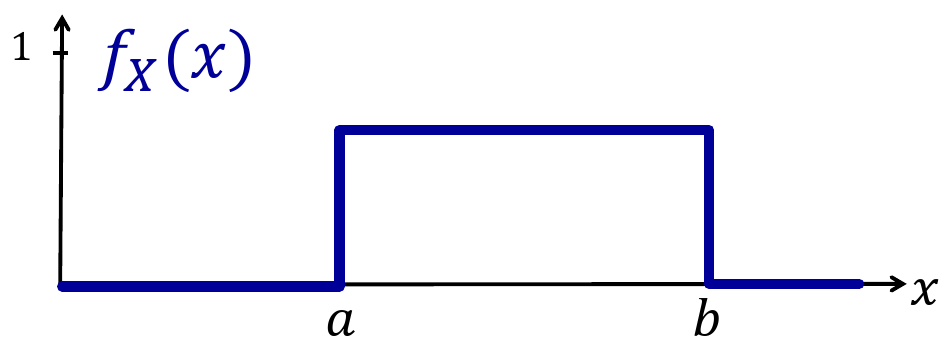
\includegraphics[scale=0.2]{images/va_uniforme}
    \label{fig_va_uniforme}
    \caption{Variable aléatoire uniforme continue}
\end{figure}
\subsubsection{Gaussienne}
La \textbf{variable aléatoire gaussienne} est très importante (pensez à la répartition de vos notes après un examen), car elle approxime très bien la somme d'un grand nombre de v.a. dont la densité de probabilité n'est pas totalement connue (très fréquent en pratique). Elle est bien connue avec sa forme de cloche, le pic se trouvant à la valeur la plus probable. Ses propriétés sont les suivantes :
\begin{enumerate}[label=P\arabic*.]
    \begin{multicols}{2}    
        \item \label{enumitem_vaGaussienne_parametres}Ses paramètres sont $(\mu,\sigma)$
        \item $f_X(x) = \frac{1}{\sigma\sqrt{2\pi}}e^{-\frac{(x-\mu)^2}{2\sigma^2}}$
        \item \label{enumitem_vaGaussienne_fRepartition}$F_X(x) = \frac{1}{2\pi} \int_{-\infty}^{-\frac{x-\mu}{\sigma}} e^{-t^2/2} \deriv t$
        \item \label{enumitem_vaGaussienne_moyVar}$\mu_X = \mu,\quad \sigma_x^2 = \sigma^2$
    \end{multicols}
        %\item $\sigma_X^2 = \frac{1}{\sigma\sqrt{2\pi}}\infint x^2 e^{-\frac{(x-\mu)^2}{2\sigma^2}} \deriv - \mu^2 = ... = \sigma^2$
    \item $\Phi_X(\omega) = \infint \frac{1}{\sqrt{2\pi\sigma^2}} \exp\(-\frac{(x-\mu)^2}{2\sigma^2}\) e^{j\omega x} \deriv x = e^{j\mu\omega -\frac{\sigma^2\omega^2}{2}}$        
\end{enumerate}
Regardons un instant ces propriétés. Nous voyons via \ref{enumitem_vaGaussienne_parametres} et \ref{enumitem_vaGaussienne_moyVar} que les paramètres passés à la v.a. ne sont autres que la moyenne (le pic que la cloche) et la variance (l'écartement de la cloche). La propriété \ref{enumitem_vaGaussienne_fRepartition} quant à elle est un peu différente : l'intégrale telle quelle ne peut se résoudre de manière analytique (sans des paramètres fixés). Il faut faire l'intégrale de manière numérique pour trouver la fonction de répartition, et elle peut ne pas exister. 

Une v.a. normale est en fait une v.a. gaussienne normalisée (i.e. $\mu = 0$ et $\sigma=1$).

\subsubsection{Exponentielle (Lambda)}
La \textbf{variable aléatoire exponentielle} mesure le temps s'écoulant entre 2 événements successifs dans un processus de Poisson de taux $\lambda$. Nous listons à nouveau ses propriétés :
\begin{multicols}{2}
    \begin{itemize}
        \item $S_X = [0,\infty[$
        \item Paramétrisée par $\lambda \in \R_+^*$
        \item $f_X(x) = \lambda e^{-\lambda x}$
        \item $F_X(x) = 1-e^{-\lambda x}$
        \item $\mu_X = \frac{1}{\lambda}$
        \item $\sigma_X^2 = \frac{1}{\lambda^2}$
        \item $\Phi_X(\lambda) = \int_0^\infty \lambda e^{-\lambda x} e^{j\omega x} \deriv x = \frac{\lambda}{\lambda - j\omega}$
        \item Elle est sans mémoire : \[P(X > t+T | X>t) = P(X>t)\]
    \end{itemize}
\end{multicols}

\subsubsection{Gamma}
Avant de parler de la v.a. gamma, nous devons parler de la fonction $\Gamma(\cdot)$, définie pour $u > 0$ :
\begin{equation}
    \Gamma(u) = \int_0^\infty x^{u-1} e^{-x} \deriv x
\end{equation}
Qui a des propriétés aux allures bien étranges :
\begin{multicols}{3}
    \begin{itemize}
        \item $\Gamma(1/2) = \sqrt{\pi}$
        \item $\Gamma(u + 1) = u\Gamma(u)$
        \item $\Gamma(u) = (u-1)!$ si $u \in \N$
    \end{itemize}
\end{multicols}
Avec ceci nous sommes en mesure de définir la \textbf{variable aléatoire Gamma} $G(\lambda, \alpha)$ :
\begin{multicols}{2}
    \begin{enumerate}[label=P\arabic*.]
        \item $S_X = ]0,\infty[$
        \item Paramétrisée par $\alpha,\lambda > 0$
        \item \label{enumitem_gamma_pdf}$f_X(x) = \frac{\lambda(\lambda x)^{\alpha -1} e^{-\lambda x}}{\Gamma(\alpha)}$
        \item $\mu_X = \frac{\alpha}{\lambda}$
        \item $\sigma_X^2 = \frac{\alpha}{\lambda^2}$
        \item $\Phi_X(\omega) = \frac{1}{(1-j\omega/\lambda)^\alpha}$
\end{enumerate}
\end{multicols}
La v.a. Gamma est très générale, il n'est donc pas surprenant que d'autres variables aléatoires découlent de Gamma. Par exemple, la v.a. $G(\lambda, m)$ avec $m \in \N$ est une \textbf{variable aléatoire d'Erlang}, de paramètres $(\lambda, m)$. Comme $m$ est entier, \ref{enumitem_gamma_pdf} devient 
\begin{equation}
    f_X(x) = \frac{\lambda(\lambda x)^{m-1} e^{-\lambda x}}{(m-1)}!
\end{equation}
Un cas particulier de la v.a. d'Erlang est lorsque $m = 1$, on obtient alors une variable \textit{v..a exponentielle}. 

Un autre cas particulier, et lorsque $\lambda = 1/2 et \alpha = \nu/2$ avec $\nu \in \N$, nous obtenons une \textbf{variable aléatoire Chi-carré} $\chi^2(\nu)$ à $\nu$ degrés de liberté. \ref{enumitem_gamma_pdf} devient alors 
\begin{equation}
    f_X(x) = \frac{x^{(\nu-2)/2}e^{-x/2}}{2^{\nu/2}\Gamma(\nu/2)}
\end{equation}
%%%%%%%%%%%%%%%%%%%%%%%%MODULE 2%%%%%%%%%%%%%%%%%%%%%%%%%%%%%%%
\section{Vecteurs Aléatoires}
\subsection{Paires de Variables aléatoires}
Maintenant que nous avons bien défini le concept de variable aléatoire, il est facile d'étendre la définition à une paire de v.a.
\subsubsection{Fonction de répartition jointe et marginale}
Nous avions précédemment la probabilité pour une variable $F_X(x) = P(X \leq x)$. Nous définissons maintenant la \textbf{fonction de répartition \uline{jointe}} : 
 \[F_{XY}(x,y) = = P(\{X \leq x\} \cap \{Y \leq y\}) = P(X \leq x,\ Y \leq y)\]
Avec comme propriétés : 
\begin{itemize}
	\item $F_{XY}(-\infty,y) = F_{XY}(x,-\infty) = 0$
	\item $F_{XY}(\infty,\infty) = 1$
\end{itemize}
Similairement, nous avons la \textbf{fonction de répartition \uline{marginale}} : 
\[F_X(x) = P(X \leq x)\qquad F_Y(y) = P(Y \leq y)\]
Qui est exactement le cas du chapitre précédent, à une variable. Elle est cependant définissable depuis le cas à deux variables, via ses propriétés :
\begin{enumerate}[label=P\arabic*.]
    \item $0 \leq F_{X,Y} \leq 1$
    \item $\limite{x\to -\infty} F_{XY}(x,y) = \limite{y\to-\infty} F_{XY}(x,y) = 0$ et $\llimite{x\to\infty}{y\to\infty}F_{XY}(x,y) = 1$
    \item Les fonction de répartition marginales peuvent être obtenues depuis la fonction de répartition jointe :
    \begin{align*}
        \limite{y\to\infty}F_{XY}(x,y) = P(X \leq x, Y \leq \infty) = F_X(x)\\
        \limite{x\to\infty}F_{XY}(x,y) = P(X \leq \infty, Y \leq y) = F_Y(y)\\
    \end{align*}
\end{enumerate}

\subsubsection{Densité de probabilité jointe et marginale}
La \textbf{densité de probabilité \uline{jointe}} est similaire : 
\begin{align}
	f_{XY}(x,y) = \frac{\partial^2F_{XY}(x,y)}{\partial x\partial y}\\
	f_{XY}(x,y) = \sum_{i,j}p_{ij}\delta(x-x_i)\delta(y-y_i)
\end{align}
En utilisant les impulsions de Dirac, nous trouvons les propriétés suivantes pour le cas discret :
\begin{enumerate}[resume,label=P\arabic*.]
    \item $\sum_{i,j} P(X=x_i, Y=y_i) = 1$
    \item $P(X\leq a, Y \leq b) = \somme{}{x_i \leq a,\ y_j \leq b} P(X = x_i,Y=y_i) = F_{XY}(a,b)$
\end{enumerate}
Et similairement pour le cas continu :
\begin{enumerate}[resume,label=P\arabic*.]
    \item $\infint\infint f_{XY}(x,y) \deriv x \deriv y = 1$
    \item $P(X \leq a, Y \leq b) = F_{XY}(a,b) = \int_{-\infty}^a\int_{-\infty}^b f_{XY}(x,y) \deriv x \deriv y$
    \item $P(a_1 \leq X \leq a_2, b_1 \leq Y \leq b_2) = \int_{a_1}^{a_2}\int_{b_1}^{b_2} f_{XY}(x,y)\deriv x\deriv y$\\Ceci implique que $P(x < X \leq x+\Delta x, y < Y \leq y+\Delta y) = \llimite{\Delta x \to 0}{\Delta y\to 0}{f_{XY}(x,y)\Delta x \Delta y} $
\end{enumerate}
Nous pouvons de la même manière définir la \textbf{densité de probabilité \uline{marginale}}, cas continu ou discret.
Pour le cas \textit{continu} :
\begin{equation}
\begin{array}{ll}
	f_X(x) &= \frac{\deriv F_X(x)}{\deriv x} = \frac{\deriv F_XY(x,+\infty)}{\deriv{x}} =\frac{\deriv{}}{\deriv{x}} \left[\int_{-\infty}^x\infint f_{XY}(\xi,\eta)\deriv{\xi}\deriv{\eta}\right]\\
			&=\infint f_{XY}(x,\eta)\deriv{\eta}\\
	f_Y(y) &= \infint f_{XY}(\xi,y)\deriv \xi
\end{array}
\end{equation}
En \textit{discret}, les choses sont légèrement plus simples grâce aux impulsions de Dirac :
\[\begin{array}{l}
    f_X(x) = \sum_{i,j} P(X=x_i, Y=y_i)\delta (x-x_i)\\
    f_Y(y) = \sum_{i,j} P(X=x_i, Y=y_i)\delta (y-y_i)\\
    P(X \leq a) = \sum_{x_i \leq a}\sum_j P(X=x_i,Y=y_i)\\
    P(X=a) = \sum_j P(X=a,Y=y_j)
\end{array}\]

\subsubsection{Variables aléatoires indépendantes}
Deux variables aléatoires $X,Y$ sont indépendantes si
\[F_{XY}(x,y) = F_X(x)F_Y(y)\]
d'où
\[f_{XY}(x,y) = f_X(x)f_Y(y)\]
Dans le cas discret, nous avons la même chose avec les probabilités :
\begin{equation}
    P(X=a,Y=b) = P(X=a)P(Y=b)
\end{equation}
Il devient donc facile de voir la propriété suivante :
\begin{itemize}
    \item Si $X$ et $Y$ sont des v.a. indépendantes, alors $g(X)$ et $g(Y)$ sont également indépendants : $X$
\end{itemize}

\subsubsection{Fonction de deux variables aléatoires}
Soient $X,Y$ des variables aléatoires, et $g_1(\cdot),g_2(\cdot)$ des fonction \uline{continues}. Alors nous définissons, en fonction de la densité jointe des v.a. $X,Y$ :
\[Z = g_1(X,Y)\quad W = g_2(X,Y)\]
Soient $(z,w)$ une paire de valeurs particulières que peut prendre la paire $(Z,W)$ et soient $(x_1,y_1),(x_2,y_2),...,(x_m,y_m)$ les $m$ racines respectives du système 
\[z = g_1(x,y)\quad w = g_2(x,y)\]
Rappelons que le jacobien de la transformation $(g_1(\cdot),g_2(\cdot))$ est la déterminant :
\begin{equation}
    J(x,y) = \det
    \begin{bmatrix}
        \frac{\partial g_1(x,y)}{\partial x} & \frac{\partial g_2(x,y)}{\partial x}\\
        \frac{\partial g_1(x,y)}{\partial y} & \frac{\partial g_2(x,y)}{\partial y}
    \end{bmatrix}
\end{equation}
On peut alors montrer que 
\begin{equation}
    f_{ZW}(z,w) = \sum_i \frac{f_{XY}(x_1,y_i)}{|J(x_i,_i)|}
\end{equation}
\paragraph{Fonctions linéaires}
Un cas particulier à prendre en compte est celui des fonctions linéaires :
Soient $g_1,g_2,Z,W$ définis comme précédemment, avec la particularité que nous imposons $g_i$ linéaire, autrement dit 
\begin{align*}
    z = g_1(x,y) = a_{11}x + a_{12}y + b_1\\
    w = g_2(x,y) = a_{21}x + a_{22}y + b_2
\end{align*}
Ce qui peut s'écrire sous forme vectorielle :
\[\mathbf{z} = A\mathbf{x + b}\]
En admettant que $\det(A) \neq 0$, la solution de cette équation est unique et donnée par 
\[\mathbf{x} = A^{-1}(\mathbf{z-b})\]
Le jacobien de $(x,y)$ devient alors 
\[J(x,y) = \det(A) = \det\begin{bmatrix}
    a_{11} & a_{12}\\
    a_{21} & a_{22}
\end{bmatrix}\]
Par conséquent, si le déterminant est non nul, la densité jointe de $\mathbf{Z} = (Z,W)$ peut s'exprimer en fonction de celle de $\mathbf{X} = (X,Y)$ : 
\begin{equation}
    f_{\mathbf{Z}}(\mathbf{z}) = \frac{f_{\mathbf{X}}(A^{-1}(\mathbf{z-b)})}{|\det(A)|}
\end{equation}

\paragraph{Exemple : somme de deux variables aléatoires indépendantes}
Prenons le cas de $Z = X+ Y$ avec $X \perp Y$
À l'annexe \ref{preuve_somme_va_produit_convo} se trouve la preuve complète. Notons simplement que cela revient au résultat final 
\begin{equation}
    f_Z = f_X \star f_Y
\end{equation}
C'est à dire le produit de convolution des densités de probabilité.
\subsubsection{Espérance d'une fonction de deux variables}
\todo{espérance}
Nous pouvons définir un concept important, la \textbf{covariance} :
\begin{equation}
Cov(X,Y) = E[(X-\mu_x)(Y-\mu_y)] = ... = E[XY] - E[X]E[Y]
\end{equation}
Également le \textbf{c\oe fficient de corrélation} :
\begin{equation}
	 \rho_{XY} = \frac{Cov(X,Y)}{\sigma_X \sigma_Y}
\end{equation}

\subsubsection{Transformées (fonction caractéristique jointe)}
\todo{??}

\subsection*{Rappel de la semaine passée}
Soient $X,Y$ des v.a. Nous avons que 
\[\begin{array}{l}
    F_{XY}(x,y) = P(X \leq x, Y \leq y) \longrightarrow F_X(x) = P(X \leq x) = F_{XY}(x,+\infty)\\
    f_{XY}(x,y) = \frac{\partial^2}{\partial x \partial y}F_{XY}(x,y) \longrightarrow f_X(x) = \infint f_{XY}(x,y) \deriv{y}\\
    \Phi_{XY}(\omega_1,\omega_2) = E[e^{j(\omega_1 X + \omega_2 Y)}] = \iint_{-\infty}^{\infty} f_{XY}(x,y)e^{j(\omega_1 X + \omega_2 Y)} \deriv{x}\deriv{y} \longrightarrow \Phi_X(\omega) = E[e^{j\omega x}] = \Phi_{XY}(\omega,0)
\end{array}\]
\subsubsection{Densité de probabilité conditionnelle}
Deux cas sont possibles comme toujours. Pour le cas \textit{discret} : 
\todo{faire les deux cas}

\subsubsection{Espérance conditionnelle}
\begin{align}
    	E[X|y] = \infint x f_{X|Y}(x|y) \deriv{x}\\
    	E[X|y] = \somme{}{i}xP(X=x_i|Y=y)
\end{align}
Notons que $E[X|y]$ est une fonction déterministe de $y$. On pourrait dire que $E[X|y] = g(y)$, ce qui implique que $E[X|Y] = g(Y)$ est une v.a. ! Cela revient à ne pas figer $Y$, et l'on peut ainsi calculer l'espérance de $g(Y)$, et donc de $E[X|Y]$ :
\begin{equation}
	\begin{array}{ll}
            E_Y[E_X[X|Y]] = \infint E[X|y]f_Y(y)\deriv y
\end{array}
\end{equation}
\todo{moar}

\subsection{Vecteurs aléatoire de dimension n}
Nous pouvons élargir tout ce que nous avons vu à $n \geq 2$
\begin{equation}
	\begin{array}{l}
            F_{X_1X_2X_3\ldots X_n}(x_1,x_2,x_3,\ldots,x_n) = P(X_1 \leq x_1, \ldots, X_n \leq x_n)
\end{array}
\end{equation}
\todo{moar}

\subsubsection{V.a. gaussiennes jointes/multivariées}
\todo{do}

\begin{equation}
	\Sigma = E[XX^T] - \mu \mu^T = \begin{bmatrix}
    \sigma_1^2 & Cov[X_1,X_2] \cdots\\
    Cov[X_2,X_1] & \sigma_2^2 \\
    \vdots & & \ddots
\end{bmatrix}
\end{equation}

Voyons le cas lorsque $m = 2$ :
\[\begin{array}{ll}
    \uline{X} \sim \mathcal{N}(\mu,\Sigma),\ \uline{X} = \begin{bmatrix}
    X_1\\ X_2
\end{bmatrix},\ \uline{\mu} = \begin{bmatrix}
    \mu_1\\ \mu_2
\end{bmatrix},\\
\Sigma = \begin{bmatrix}
    \sigma_1^2 & \rho\sigma_1\sigma_2\\
    \rho\sigma_1\sigma_2 &  \sigma_2^2
\end{bmatrix} \to \det{\Sigma} = \sigma_1^2\sigma_2^2(1-\rho^2) \to \Sigma^ {-1} = \frac{1}{\sigma_1^2\sigma_2^2(1-\rho^2}\begin{bmatrix}
    \sigma_2^2 & -\rho\sigma_1\sigma_2\\
    -\rho\sigma_1\sigma_2 & \sigma_1^2
\end{bmatrix}\\
f_{X_1X_2}(x_1,x_2) = \frac{1}{\sqrt{(2\pi)^2 \det{\Sigma}}} \exp\(\frac{-1}{2(1-\rho^2)}\left[\(\frac{x_1-\mu_1}{\sigma_1}\)^2 - 2\rho \(\frac{x_1-\mu_1}{\sigma_1}\)\(\frac{x_2-\mu_2}{\sigma_2}\) + \(\frac{x_2-\mu_2}{\sigma_2}\)^2\right]\) = k\\
\Longrightarrow \(\frac{x_1-\mu_1}{\sigma_1}\)^2 - 2\rho \(\frac{x_1-\mu_1}{\sigma_1}\)\(\frac{x_2-\mu_2}{\sigma_2}\) + \(\frac{x_2-\mu_2}{\sigma_2}\)^2 = \underbrace{-2(1- \rho^2)\ln\(k2\pi\sigma_1\sigma_2\sqrt{1-\rho^2}\)}_{K}
\end{array}\]
Pour tout $|\rho| < 1$ : le plan de hauteur $k$ qui coupera la cloche de la Gaussienne, nous pouvons déterminer la forme du cercle/elipse qui en découle. Par exemple, pour :
\begin{itemize}
    \item $\rho=0$ : $\(\frac{x_1-\mu_1}{\sigma_1}\)^2 + \(\frac{x_2-\mu_2}{\sigma_2}\)^2 = K$, ce qui, pour $\sigma_1 > \sigma_2$ donne une ellipse centrée en $(\mu_1,\mu_2)$ et avec les demis-rayons de taille $\sigma_1$ et $\sigma_2$. Si en revanche $\sigma_1 = \sigma_2 = \sigma$, nous obtenons un cercle, le centre est toujours le même.
    \item $\rho \neq 0$ nous obtenons une ellipse légèrement tournée. Plus $\rho$ tend vers 1, plus l'ellipse s'aplatit et s'approche de la droite $y=x$.
\end{itemize}
\todo{propriétés}

\subsection{Convergence d'une suite de variables aléatoires}
\subsubsection{Convergence presque sûre}
\subsubsection{Convergence en distribution et Théorème Central Limite}
\subsubsection{Convergence en probabilité et loi faible des grands nombres}
\[\forall \epsilon > 0,\ P\{|X_n - X| > \epsilon\} \to 0 \pour \ninf\]
La loi faible des grands nombres : Soit $X_1,X_2,...,X_n$ une suite de v.a. i.i.d. de moyenne $\mu$ et de variance $\sigma^2$. Alors en définissant
\[Z_n = \frac{1}{n}\somme{n}{i=1}X_i\]
Nous avons
\[\forall \epsilon > 0,\ P\{|Z_n - \mu| > \epsilon\} \to 0 \pour \ninf\]

\section{Processus Stochastiques}
\subsection{Processus stochastiques à temps continu}
\subsubsection{Définition}
Nous connaissions les variables aléatoires, qui mappaient un événement à une valeur (réelle souvent). Par exemple des probabilités sur l'âge d'une personne, ou sur la température. Les processus stochastiques rajoutent une dimension temporelle à cela. Avant on avait $X(\zeta) \to x$ avec $\zeta \in \Omega$ et $x \in \R$. Nous avons maintenant le \textbf{processus stochastique} $X(\zeta, t) \to x\in \R$. Nous pouvons échantillonner le processus $X(t,\zeta)$ aux temps $t_1,t_2,...,t_n$ afin d'avoir $n$ variables aléatoires : $X_1 = X(t_1,\zeta),\ X_2 = X(t_2,\zeta),...,X_n = X(t_n\zeta)$. Le processus stochastique est spécifié par la collection de toutes les fonctions de répartition jointes du nième ordre obtenues pour tout $n \in \N_0 = N \setminus \{0\}$ et tous les instants $t_+,...,t_n \in \R$

Cependant ici nous ne parlerons que des deux premiers ordres, donc la moyenne
\[\mu_X(t) = E[X(t)] = \infint xf_X(x;t)\deriv x\]
Notons qu'il ne s'agit plus ici d'une valeur fixe mais d'une fonction : la moyenne en fonction du temps 
\begin{exemple}
    Précédemment, nous avions l'espérance de la température, mais ici nous avons la moyenne de température à chaque instant de la journée : la moyenne à midi est différente de celle à 15h.
\end{exemple}
Pour l'ordre 2, nous avons la \textit{fonction d'auto-corrélation} :
\[R_X(t_1,t_2) = E[X(t_1)X(t_2)] = \infint\infint x_1x_2f_{X(t_1)X(t_2)}(x_1,x_2;t_2,t_2)\deriv x_1 \deriv x_2\]
Et de manière similaire la \textit{fonction d'auto-covariance} :
\[C_X(t_1,t_2) = E[(X(t_1)-\mu_X(t_1))(X(t_2) - \mu_X(t_2))] = R_X(t_1,t_") - \mu_X(t_1)\mu_X(t_2)\]
\subsubsection{Exemples}
\paragraph{Sinusoïde à phase aléatoire} 
    \[X(t) = a\sin(2\pi f_0 t + \Phi(\zeta))\]
    Avec $a,f_0$ constants et $\Phi(\zeta)$ une v.a. de Bernoulli : \[\Phi(\zeta) = \left\{\begin{array}{ll}
    0 & \text{a.p. }1/2\\
    \pi &\text{a.p. } 1/2
\end{array}\right.\]
Autrement dit avec probabilité égale, soit $\Phi=0$ et $X(t) = a\sin(2\pi f_0 t)$ ou $\Phi=\pi$ et $X(t) = a\sin(2\pi f_0 t + \pi) = -a\sin(2\pi f_0 t)$. Nous avons donc un graph $t\to X(t)$, sur lequel nous avons deux sinusoïdes : un sinus et un sinus inversé.

Prenons nos deux ordres :
\begin{align*}
    \mu_X(t) = E[X(t)] = E[X(t) | \Phi = 0]P(\Phi = 0) + E[X(t) | \Phi=\pi]P(\Phi=\pi)\\
     = \frac{1}{2}\left[a\sin(2\pi f_0 t) - a\sin(2\pi f_0 t)\right] = 0
\end{align*}
Similairement, la fonction d'auto-corrélation :
\[\begin{array}{ll}
    R_X(t_1,t_2) &= E[X(t_1)X(t_2)] \\ &= E[X(t_1)X(t_2)|\Phi=0]\frac{1}{2} +E[X(t_1)X(t_2)]\\ &= E[X(t_1)X(t_2)|\Phi=\pi]\frac{1}{2}\\ &= \frac{1}{2}a^2\sin(2\pi f_0 t_1)\sin(2\pi f_0 t_2) + \frac{1}{2}a^2\sin(2\pi f_0 t_1)\sin(2\pi f_0 t_2)\\ &= a^2\(\cos(2\pi f_0 (t_+-t_2)) - \cos(2\pi f_0 (t_1+t_2)\)
\end{array} \]
\paragraph{Nouveau Phi} 
   Reprenons l'exemple précédent avec $\Phi \sim U(0,2\pi)$ (donc $x = \frac{1}{2\pi}$ entre 0 et $2\pi$, 0 partout ailleurs). La moyenne :
    \[\mu_X(t) = E[X(t)] = \int_0^{2\pi} a\sin(2\pi F_0 t + \phi)\frac{1}{2\pi} \deriv \phi = 0\]
\paragraph{Processus gaussien}
    $X(t)$ est un processus gaussien si chaque v.a. $X(t_1),X(t_2),...,X(t_n)$ sont des v..a gaussiennes jointes. Comme vu au module 2 (voir ????), il est donc entièrement spécifié par sa moyenne et sa fonction de covariance. Rappelons sa densité jointe de probabilité :
    ???
    avec ?????
\todo{rajouter ref}
\todo{mettre le bordel}
\paragraph{Processus Markovien}
Un processus $X(t)$ tel que pour tout \todo{compléter}

\paragraph{Processus à accroissements indépendants}    

\paragraph{Processus de Wiener}
(pas utile pour le moment)

\paragraph{Processus de Poisson}
Rappel sur Poisson : $X \sim P(\lambda)$ discrète. Nous avons $P(X=k) = \frac{\lambda^k}{k!}e^{-\lambda}$ \todo{rajouter détails}. Nous calculons sa moyenne : 
\[\mu_X(t) = \lambda t\]

\paragraph{Martingale}

\paragraph{Modulation d'amplitude de pulse (PAM)}
Un des signaux les plus importants en communication numérique : une suite de ``pulses'' $\{g(t-kT),k\in \Z\}$, modulée en amplitude par la suite de variables aléatoires $\{A_k, k \in \Z\}$ et $T$ une constante ($\simeq$ période)
\begin{equation}
    X(t) = \somme{\infty}{-\infty} A_k g(t-kT)
    \label{equ:PAM}
\end{equation}


Nous faisons plusieurs hypothèses : \todo{hypothèses}

\subsubsection{Stationarité}
\paragraph{Stationnarité au sens strict et au sens large}~

Un processus stochastique $X(t)$ est \textbf{stationnaire} (\textit{au sens strict}) (SSS) si et seulement si toutes ses propriétés stochastiques sont indépendantes de l'origine des temps. Donc $\forall n \in \N_0,\ t_1,t_2,...,t_n \in \R$ et $c \in \R$
\[F_{X(t_1),...,X(t_n)}(x_1,...,x_n;t_1,...,t_n) = F_{X(t_1+c),...,X(t_n+c)}(x_1,...,x_n;t_1+c,...,t_n+c)\]

\[\mu_X(t9 = E[X(t)] = \infint x f_{X(t)} (x,t)\deriv x = \infint x f_{X(t+c)}(x;t+c) \deriv x = E[X(t+c)] = \mu_x(t+c)\]
\[R_X(t_1,t_2) = \infint\infint x_1x_2 f_{X(t_1)X(t_2)}(x_1,x_2;t_1,t_2)\deriv x_1 \deriv x_2 = \infint\infint x_1x_2f_{X(t_1+c)X(t_2+c)}(x_1,x_2;t_2,t_2) \deriv x_1 \deriv x_2 = R_X(t_1+c,t_2+c) = R_X(t_1-t_2)\]
Si la moyenne ne dépend pas du temps, et la fonction d'auto-corrélation ne dépend que de la diférence entre les deux isntants auxquels elle est évaluée (ci-dessus) alors elle est dit \textbf{stationnaire au sens large} (WSS). Notons que $SSS \to WSS$.

\paragraph{Exemples}
\begin{itemize}
    \item $X(t) = A \cos(2\pi f_0 t) + B \sin(2\pi f_0 t)$ avec $A \indep B,\ \mu_A = \mu_B = 0, \sigma_A^2 = \sigma_B^2 = 1$. Nous trouvons que $\mu_{X(t)} = 0 = \mu_X$ et $R_X(t_1,t_2) = \cos(2\pi f_0(t_1-t_2)) = R_X(t_2-t_2)$, donc il est WSS
    \item Même exemple, mais avec $A \sim \mathcal{N}(0,1)$ et $B\sim unif[-\sqrt{3\pi},\sqrt{3\pi}]$. Si $t=0$, on a $X(t=0) = A$ mais pour $t=\frac{1}{4f_0} \to X(t=\frac{1}{4f_0} = B$. Donc $P(X(0) \leq x) \neq P(X(\frac{1}{4f_0} \leq x)$ donc il n'est pas WSS. 
    \item $X(t) = a \cos(2\pi f_0 t + \Phi),\ \Phi \sim unif[0,2\pi]$. on calcule $\mu_X(t) = 0$ et $R_X(t_1,t_2) = \frac{a^2}{2} \cos(2\pi f_0(t_1-t_2))$
\end{itemize}

\subsubsection{Ergodisme}
La semaine prochaine. Voir \ref{subsubsec:ergodisme}.
\subsubsection{Densité spectrale}
Soit $X(t)$ WSS (donc $R_X(t,t-\tau) = R_X(\tau)$). Alors on définit
\begin{equation}
    S_X(f) = \infint R_X(\tau) e^{-2\pi j f \tau} \deriv \tau
\end{equation}
Bien définie si
\[\infint |R_X(\tau)| \deriv \tau < \infty\]
Il est de plus possible d'obtenir la fonction d'auto-corrélation par la transformée inverse :
\begin{equation}
    R_X(\tau) = \infint S_X(f) e^{j2\pi f\tau}\deriv f
\end{equation}
En particulier, la puissance des moyennes de $X(t)$ est :
\begin{equation}
    E[X^2(t)] = R_X(0) = \infint S_X(f)\deriv f
\end{equation}
Les jolies propriétés suivantes :
\begin{enumerate}[label=P\arabic*.]
    \item Si $X(t)$ est WSS, alors $R_X(\tau)$ est paire :
    \[R_X(\tau) = E[x(t)x(t-\tau] = E[x(t-\tau)x(t)] = R_X(-\tau)\]
    \item $S_X(f) \geq 0$
    \item La fonction $h(f) = S_X(f)/R_X(0) \geq 0$ est une densité de probabilité, car
    \[\infint h(f)\deriv f = \frac{1}{R_X(0)}\infint S_X(f) \deriv f = \frac{R_X(0)}{R_X(0)} = 1\]
\end{enumerate}

\subsubsection{Exemples}
\begin{itemize}
    \item Sinusoide
    \item Bruit blanc : processus stochastique WSS dont la densité spectrale de puissance est constante : $\frac{N_0}{2}$ pour toutes les fréquences :
    \[S_N(f) = \frac{N_0}{2}\]
\end{itemize}

\subsubsection{Ergodisme}
\label{subsubsec:ergodisme}
Un processus qui va explorer toutes les valeurs que l'espace des valeurs peut prendre. Si nous prenons un processus $X(t) = \{x(t), t\in \R\}$ \textit{wss}. Sa moyenne est bien entendu définie par $\mu_X = \mathrm{E}[x(t,\zeta)] = \somme{}{i} x_i P(X=i)$. Cette moyenne peut être estimée par la moyenne \textit{temporelle} d'une de ces réalisations $x(t)$ : 
\[< x(t) >_T = \frac{1}{T}\int_0^T X(t) \deriv t\]
Au lieu de prendre une \todo{définition}

\begin{exemple}
    Prenons un sac de monnaie (aliage métal-nickel) mais certaines biaisées : certaines ont un côté face en plomb, et certaines l'ont en aluminium. 0 si face, 1 si pile. 
    
    Là deux manières de faire : si on prend une pièce (disons plombée) et la tirons plusieurs fois, on aura un graphe biaisé (plus souvent pile, donc plus souvent 1). Si on tire souvent une pièce en aluminium, le graphe sera biaisé inversement. Mais ce qui est intéressant est qu'en tirant plus de fois cette même pièce, on n'aura pas un indicateur plus stable, la pièce reste fausse. Si la même pièce est jouée successivement à pile ou face, on aura $<x>_T \neq \mu_X$. En d'autres termes, en prenant une trajectoire "alu" on aura un biais, en prenant une trajectoire "plomb" elle sera aussi biaisée (inversement). Il est donc intéressant de prendre une pièce au hasard à chaque tirage.
\end{exemple}

Notons que $<x>_T$ est défini comme l'intégrale d'une v.a., c'est donc aussi une v.a. Nous remarquons aussi que 
\[E[<x>_T] = E[\frac{1}{T}\int_0^T x(t)\deriv t] = \frac{1}{T}\int_0^T E[x(t)] \deriv t = \frac{1}{T}\mu_X T = \mu_X\]

 \begin{suiteExemple}
    En continuant avec notre sac, nous trouvons 
    \[E[<x>_T] = \underbrace{E[<x>_T|Pb]}_{9/10}\underbrace{P(Pb)}_{1/2} + \underbrace{E[<x>_T|Al]}_{1/10} \underbrace{P(Al)}_{1/2} = 1/2 = \mu_X\]
\end{suiteExemple}
Notons également que 
\[\limite{T\to\infty} VAR[<x(t)>_T] = \limite{T\to\infty}E[<x(t)>_T - \mu_X)^2] = 0\]

\todo{???}

\paragraph{Exemples}
\begin{itemize}
    \item Signal P.A.M : sa définition est à l'équation \ref{equ:PAM}. Notons le cas particulier $A_k \in \{-1,1\}$ i.i.d. et $D \sim U[0,T]$. Nous calculons
     \[\mu_X(t) = E[\somme{+\infty}{k=-\infty} A_k g(t-kT-D)] = \somme{+\infty}{k=-\infty} \underbrace{E[A_k]}_0 E[g(t-kT-D)] = 0\]
     \begin{align}
    R_x(t_1,t_2) = E[\somme{+\infty}{k=-\infty} A_k g(t_1-kT-D) \somme{+\infty}{=-\infty} A_l g(t_2-lT-D)]\\ = \somme{+\infty}{k=-\infty}\somme{+\infty}{l=-\infty} E[A_k A_l]E[ g(t_+-kT-D)g(t_2-lT-D)]\\
    \forall l\neq k\ :\ E[A_kA_l] = E[A_k]E[A_l]= 0\quad k=l\ E[A_kA_l] = E[A_k^2] = 1
\end{align}
Prenons la seconde espérance (en prenant le cas particulier où $l=k$) :
\begin{align}
    E[ g(t_+-kT-D)g(t_2-lT-D)] = \int_0^Tg(t_+-kT-s)g(t_2-lT-s) \frac{1}{T}\deriv s
\end{align}
Le tout vaut donc
\[\frac{1}{T}\somme{k=-\infty}{+\infty} \int_0^T g(t_1-kT-s)g(t_2-kT-s) \deriv s \]
On place le changement de  variable $s' = t_1-k_T-s$ donc $s=t_1-kT-s'$ on trouve
\[=\frac{1}{T} \somme{\infty}{k=-\infty} \int_{t_1-(k+1)T}^{t_1-kT} g(s')g(s'+t_"-t_1) \deriv s' = \frac{1}{T} \infint g(s')g(s'+t_2-t_1)\deriv s'\]
\end{itemize}

\subsection{Application 1 : Distorsion de fréquence en radiocomunication avec un mobile}
Pas fait

\subsection{Application 2 : Taux d'erreur d'un signal PAM}


\section{Processus stochastiques à temps discret : analyse au second ordre}
    
\begin{sidewaystable}
    \begin{tabular}{c|c}
    Processus Stochastique à valeurs réelle et temps réel & Processus Stochastique à valeurs réelle et temps discret\\
    &$F_{X_1...,X_m}(x_1,...,x_m;n_1,...,n_m) =P(X(n_1) \leq x_1;...;X(n_m) \leq x_m)$
\end{tabular}
\end{sidewaystable}

\section{Processus de Poisson}
\subsection{Poisson sur R+}
\subsubsection{Processus de comptage}
Un processus stochastique $\{N(t), t\in \R^+\}$ (donc à temps continu positif) est appelé un \textbf{processus de comptage} si $N(t)$ représente le nombre d'événements se déroulant dans l'intervalle de temps $[0,t]$ avec les propriétés suivantes :
\begin{itemize}
    \item Processus à temps continu et à valeurs entières non négatives
    \item $N(0) = 0$ (totalement arbitraire)
    \item $t_1 < t_2$ alors $N(t_1) \leq N(t_2)$
    \item Le nombre d'événements dans l'intervalle $]t_1,t_2]$ est donné par $N(t_2) - N(t_1)$
\end{itemize}
A ce processus de comptage sont associés \textbf{la séquence des temps d'arrivée} $\{S(n), n \in \N_0\}$ qui décrit le temps où se produit l'arrivée du $n$ième événements, et \textbf{la séquence des temps entre arrivées} $\{T(n), n \in \N\}$ qui décrit l'intervalle de temps séparant l'arrivée du nième et du $(n+1)$ième événement. 

Ces processus sont liés par les relations suivantes : 
\begin{align}
    N(t) \geq n \iff S(n) \leq t\\
    S(n) = \somme{n-1}{m=0}T(m)\\
    T(n) = S(n+1) - S(n)
\end{align}
On peut redéfinir $S(n)$ : 
\begin{align}
    N(t) =  \max\{n \in \N_0 : S(n) \leq t\}\\
    S(n) = \inf\{t \in \R^+ : N(t) = n\}
\end{align}

\subsubsection{Définition et loi de probabilité d'un processus de Poisson}
Une première définition du processus de Poisson homogène est la suivante :

\evid{Définition 1} Un processus de Poisson homogène d'intensité $\lambda > 0$ est un processus de comptage qui satisfait aux trois hypothèses suivantes :
\begin{enumerate}[label=H\arabic*.]
    \item Le processus est à accroissement indépendants : des événements se déroulant dans des intervalles de temps disjoints sont indépendants, i.e.
    \[P(\{N(t+T) - N(t) = n_0\} \cap \{N(t) = n_1\}) = [P(N(t+T) - N(t) = n_0)P(N(t) = n_1)\]
    \item Le processus est homogène dans le temps, i.e. ses accroissements sont stationnaires : le nombre d'événements se déroulant dans un intervalle de temps ne dépend que de la longueur.
    \[P(N(t+T) - N(t) = n_0) = P(N(T) = n_0)\]
    \item La probabilité que deux événements ou plus se produisent dans un petit intervalle de temps $\Delta t$ est négligeable par rapport à la probabilité qu'il n'y ait qu'un seul événement. Plus précisément : 
    \begin{align*}
        P(N(\Delta t) = 1) = \lambda\Delta t + o(\Delta t)\\
        P(N(\Delta t) \geq 2) = o(\Delta t)
    \end{align*}
\end{enumerate}

Une manière alternative de définit le processus : 

\evid{Définition 2} Un processus de Poisson homogène d'intensité $\lambda > 0$ est un processus de comptage qui satisfait aux deux hypothèses suivantes :
\begin{enumerate}
    \item Le processus est à accroissements indépendants
    \item Le nombre d'événements se déroulant dans un intervalle de temps de longueur $T$ suit une loi de poisson, i.e. pour tout $t,\ T \geq 0$ et $n \in \N$ 
    \[P(N(t+T) - N(t) = n) = \frac{(\lambda T)^n}{n!}    e^{-\lambda T}\]
\end{enumerate}

Ces deux définitions sont parfaitement équivalentes, comme prouvé à l'annexe \ref{preuve_egalite_definitions_processus_poisson}.

Il est intéressant de calculer leur transformée en Z : 
\[\begin{array}{ll}
    \limite{\Delta t \to 0}{\frac{p_n(t+ \Delta t) - p_n(t)}{\delta t}} = -\lambda p_n(t) + \lambda p_{n-1})(t) + \frac{o(\Delta t)}{\Delta t} \somme{n}{k=0} p_{n-k}(t)\\
    z^n \frac{d p_n(t)}{dt} = -\lambda z^n p_n(t) + \lambda z^n p_{n-1} & n \geq 1\\
    z^0 \frac{d p_0}{dt}(t) = -\lambda z^0 p_0(t)\\
    \somme{\infty}{m=0} z^n \frac{dp_m}{dt}(t) = -\lambda \somme{\infty}{m=0} z^m p_m(t) + \lambda z \somme{\infty}{m=1} z^{m-1}p_{m-1}(t) \overset{l=m-1}{1} -\lambda \somme{\infty}{m=0} z^m p_m(t) + \lambda z \somme{\infty}{l=0} z^{l}p_{l}(t)\\
    \frac{d}{dt}\somme{\infty}{n=0} z^n p_n(t) = \lambda(z-1) \somme{\infty}{n=0}p_n(t)\\
    \frac{d}{dt}G_{N(t)}(z;t) = \lambda(z-1) G_{N(t)}(z;t) \to G_{N(t)} = G_N(z;0) e^{\lambda t(z-1)} = e^{\lambda t(z-1)}
\end{array}\]
\subsubsection{Propriétés}
Ainsi $N(t)$ est une v.a. de Poisson, dont la fonction génératrice est calculée ci-dessus. Sa moyenne est 
\[\mu_N(t) = E[N(t)] = \lambda t\]
Avec une variance
\[\sigma_N^2(t) = E[N^2(t)] - \mu_N^2(t) = \lambda t\]

Sa fonction d'auto-corrélation est 
\[\begin{array}{llll}
    R_N(t_1,t_2) &= E[N(t_1)N(t_2)] \neq E[N(t_1)]E[N(t_2)] & & \text{car} \not\indep\\
    &= E[N(t_1) [N(t_2) - N(t_1) + N(t_1)]] \\
    &= E[N(t_1)\big(N(t_2)-N(t_1)\big) + N^2(T_1)]\\
    &= E[N(t_1)\big(N(t_2)-N(t_1)\big)] + E[N^2(T_1)]\\
    &=\underbrace{E[N(t_1)]}_{\lambda t_1} \underbrace{E[N(t_2) - N(t_1)]}_{\lambda(t_2-t_1)} + \underbrace{E[N^2(t_1)]}_{\lambda^2 t_1^2 + \lambda t_1}\\
    &=\lambda^2 t_1t_2 - \lambda^2 t_1^2 + \lambda^2 t_1^2 + \lambda t_1 & = \lambda t_1 + \lambda^2 t_1 t_2 & t_1 \leq t_2\\
    && =\lambda t_2 + \lambda^2 t_1 t_2 & t_2 \leq t_1\\
    &= \lambda^2 t_1 t_2 + \lambda \min\{t_1,t_2\}
\end{array}\]

La \textit{superposition} de $M$ processus de Poisson indépendants $N_i(t)$ de taux $lambda_1,\ 1\leq i\leq M$ est encore un processus de Poisson $N(t)$ de taux $\lambda = \sum_{i=1}^M \lambda_i$

\subsubsection{Séquence des temps d'arrivée et inter-arrivées}
La \textit{séquence des temps d'arrivée} $\{S(n), n\in \N_0\}$ suit une loi d'Erlang :
\todo{add}

La \textit{séquence des temps entre arrivées} $\{T(n), n \in \N\}$ est une suite de v.a. exponentielles i.i.d. :
\[\begin{array}{lll}
    P(T(0) > t) &= P(N(t) = 0) = e^{-\lambda t}\\
    F_{T(0)}(t) &= P(T(0) \leq 1) = 1- e^{-\lambda t}\\
    f_{T(0)}(t) &= \lambda e^{-\lambda t} & t\geq 0\\
    P(T(n) > t) &= P(S(n+1) - S(n) > t)\\
                &= P(S(n+1) - S(n) > t | S(n) = s)\\
                &= P(N(t+s) - N(s) = 0 | S(n) = s)\\
                &= P(N(t+s) - N(s) = 0)\\
                &= P(N(t) = 0) = e^{-\lambda t}
\end{array}\]

\subsection{Processus et bruit impulsif de Poisson sur R}
\subsubsection{Processus de Poisson sur R}
On décide maintenant de regarder les temps négatifs (on étend notre définition). Logiquement, les valeurs $N(t)\ t < 0$ seront négatives. Nous pouvons donc redéfinir :
\begin{equation}
    T(n) = S(n+1) - S(n)\qquad T(0) = S(1) - S(0)
\end{equation}

\subsubsection{Bruit impulsif de Poisson (Shot noise)}
Le processus stochastique
\begin{equation}
    X_h(t) = \somme{\infty}{n=-\infty} h(t- S(n))
\end{equation}
avec $h(t)$ une fonction déterministe, et $\{S(n), n \in \Z\}$. $X_h(t)$ est appelé \textbf{bruit impulsif de Poisson}. Dans le cas particulier où 
\[h(t) = 1_{\R_0^+}(t) = \left\{\begin{array}{ll}
    1 & \text{si } t > 0\\
    0 & \text{si } t \leq 0
\end{array}\right.\]
Alors ce processus est le processus de Poisson défini plus tôt. 

Nous prenons la dérivée, grâce à Dirac :
\[X_{\delta}(t) = \somme{\infty}{n=-\infty} \delta(t-S(n))\]
et en appliquant $h(t)$
\[X(t) = (h \star X_\delta)(t)\]

Mettons cela formel. Pour tout processus $Y(t)$ de moyenne $\mu_Y(t)$ et de foncion d'auto-corrélation $R_X(t_1,t_2)$. Alors :
\[Y'(t) = \frac{\deriv Y}{\deriv t}(t)\]
Alors
\begin{align*}
    \mu_{Y'}(t) = E[Y'(t)] = \frac{\deriv \mu_Y}{\deriv t}(t)\\
    R_{Y'}(t_1,t_2) = E[Y'(t_1)Y'(t_2)] = \frac{\partial^2 R_Y}{\partial t_1 \partial t_2}(t_1,t_2)
\end{align*}
Dans le cas particulier $h(t) = \delta(t)$ :
\[Y_\delta(t) = \frac{\deriv Y_{1_{R_0^+}}}{\deriv t}(t) = \frac{\deriv N}{\deriv t}(t)\]
Et pour $Y(t) = N(t)$ :
\begin{align*}
    E[N(t)] = \lambda t \to E[\frac{d}{dt}N(t)] = \lambda\\
    R_N(t_1,t_2) = \lambda^2 t_1t_2 + \lambda \min\{t_1,t_2\}\\
     \to R_{N'}(t_1,t_2) = \frac{\partial^2}{\partial t_1 \partial t_2}[\lambda^2 t_1t_2 + \lambda \min\{t_1,t_2\} = \lambda^2 + \underbrace{\lambda \frac{\partial^2}{\partial t_1 \partial t_2} \min\{t_1,t_2\}}_{\delta(t_1-t_2)}
\end{align*}

Alors $X_\delta(t) = N'(t) = \frac{\deriv N}{\deriv t}(t) = \lambda^2 +\lambda\delta(t_1-t_2)$. Donc $X_\delta(t)$ est WSS, donc on peut calculer sa densité spectrale de puissance :
\[S_{X_\delta}(f) = \lambda^2\delta(f) + \lambda\]

\paragraph{Rappel, début de semaine 7}
Nous partons des temps d'arrivée d'un processus de Poisson de taux $\lambda$ caractérisée par $\{S(n), n \in \Z\}$. A chaque arrivée nous avons une impulsion, en général qui décroit en forme $e^{-x}$. Ensuite nous avons $x$ la somme de ces courbes :
\[x_h(t) = \somme{\infty}{n=-\infty} h(t-S(n))\]
Nous avons ensuite trouvé le théorème de Campbell :
\[\mu_{x_h} = \lambda \infint h(t) \deriv t \qquad \sigma^2_{x_h} = \lambda \infint h^2(t) \deriv t\]
\paragraph{Revenons à nos moutons}
\subsection{Application : rapport signal/bruit d'un photodétecteur (fibre optique)}
Un signal est converti, grâce à un laser, en un signal optique. La théorie quantique prédit que le processus des arrivées des photons est un processus de Poisson. Mais la charges mettent un temps à parcourir la zone de déplétion de la diode, si bien que nous avons un bruit (impulsif de Poisson) :
\[I_i(t) = e \sum_n h(t-S'(n))\]
Nous avons aussi un courant d'obscurité $I_d(t)$ :
\[I_d(t) = e \sum_n h(t-S''(n))\]
Le nombre moyen de paires de charges est proportionnel à la puissance optique incidente $P_s(t)$. Avec $h\nu$ la constante de Planck et $\mu$ la fréquence optique :
\[\lambda_i = \frac{\eta P_s}{h\nu}\]
Le courant d'obscurité a une intensité $\lambda_d$. Comme les deux processus de Poisson sont indépendants, nous leur somme est un processus de Poisson d'intensité $\lambda = \lambda_i + \lambda_d$ avec $\{S(n)\} = \{S'(n)\} \cup \{S''(n)\}$. Le courant total est converti en tension :
\[V(t) = g(I_i(t) + I_d(t)) = ge\sum_n h(t-S(n))\]
A cette tension s'ajoute une tension de bruit thermique $V_{th}(t)$ (à moyenne nulle et variance $\sigma^2_{th}$) :
\[V_{out}(t) = ge \sum_n h(t-S(n)) + V_{th}(t)\]
Le rapport signal sur bruit de la photodiode est défini par (avec $P_s$ constant) :
\begin{equation}
    SNR = \frac{E^2[V(t)|\lambda_d=0]}{VAR[V_{out}(t)}
\end{equation}
Grâce à Campbell nous trouvons
\begin{align}
    E[V(t)|\lambda_d = 0] = ge \lambda_i \infint h(s)\deriv s = \frac{\eta g e P_s}{h\nu}\infint h(s)\deriv s\\
    VAR[V_{out}(t) = g^2 e^2 \(\frac{\eta P_s}{h\nu}+\lambda_d\) \infint h^2(s) \deriv s + \sigma^2_{th}
\end{align}
Ce qui donne :
\begin{equation}
    SNR_{PIN} = \frac{\(\(\frac{\eta P_s}{h\nu}\)\infint h(s)\deriv s\)^2}{\(\frac{\eta P_s}{h\nu} + \lambda_d\)\infint h^2(s) \deriv s + \frac{\sigma^2_{th}}{g^2e^2}}
\end{equation}



%%%%%%%%%%%%%%%%%%%%%%%%%%%%%%%%%%%%%%%%%%%%%%
%%%%%%%%%%%%%%%    Module 6     %%%%%%%%%%%%%%
%%%%%%%%%%%%%%%%%%%%%%%%%%%%%%%%%%%%%%%%%%%%%%
\section{Chaines de Markov à temps discret}
Un processus est dit \textit{Markovien} si l'évolution du processus ne dépend que de sa valeur actuelle et non des valeurs passées. Plus précisément, si $X(t)$ est à valeur discrète, il est Markovien et est appelé \textit{chaîne de Markov} ssi pour toute suite d'instants $t_1<t_2<...<t_k<t_{k+1}$ et toute suite de valeurs $x_1,x_2,...,x_k,x_{k+1}$ :
\begin{equation}
    P(X(t_{k+1}) | X(t_1)=x_1,...,X(t_k) = x_k) = P(X(t_{k+1}) | X(t_k) = x_k)
\end{equation}
Toutes les valeurs que $X(t)$ peut prendre est appelé \textit{l'espace d'état}. Si l'espace d'état est discret, il s'agit d'une \textbf{chaîne de Markov} (à temps discret ou continu, en fonction de $t$), sinon on parle d'un \textbf{processus de Markov}, ssi \todo{grosses formules}

\subsection{Chaînes de Markov à temps discret}
Ici, l'espace d'état $\mathcal{S}$ est dénombrable, fini ou non. 
\subsubsection{Probabilités d'état et de transition}
La probabilité que $X(n)$ soit dans l'état $i \in \mathcal{S}$ est une des \textbf{probabilités d'état} $\pi_i(n) = P(X(n) = i)$ avec comme propriété intéressante que 
\begin{equation}
    \sum_{i\in \mathcal{S}} \pi_i(n) = 1
\end{equation}
Alors que les probabilités $p_{ij}(n) = P(X(n+1) = j | X(n) = i)$ sont appelés les \textbf{probabilités de transition à une étape} de l'état $i$ à $j$ au temps $n$, qui satisfait la relation 
\begin{equation}
    \sum_{j \in \mathcal{S}} p_{ij}(n) = 1
\end{equation}
Dès maintenant, nous supposons qu'elles ne dépendant pas du temps $n$ (on dit que la chaîne est \textbf{homogène}). On peut aussi les écrire sous la forme d'une \textbf{matrice de transition} ou \textbf{matrice stochastique} :
\begin{equation}
    P = 
        \begin{bmatrix}
            p_{00} & p_{01} &\cdots & p_{0i}& \cdots\\
            p_{10} & p_{11} & \cdots & p_{1i} & \cdots\\
            \vdots & \vdots & \ddots & \vdots\\
            p_{i0} & p_{i1} & \cdots & p_{ii} & \cdots\\
            \vdots & \vdots & & \vdots & \ddots
        \end{bmatrix}
\end{equation}
Dont la somme des éléments d'une ligne valent toujours 1. 

Il est ensuite intéressant de calculer les \textbf{probabilités de transition à 2 étapes} de l'état $i$ à l'état $j$ :
\[\begin{array}{ll}
    p_{ij}^{(2)}   &= P(X(n+1) = j | X(n) = i) \\
                   &= 
\end{array}\]
\todo{compléter}

\subsubsection{Classification des états}
\paragraph{Classe / chaîne irréductible}
\begin{itemize}
    \item Un état $j$ est \textbf{accessible} à partir de $i$ si $\exists m \in \N_0:\ p_{ij}^{(m)} > 0$, donc il existe une suite de transition (possibles) pour passer de $i$ à $j$.
    \item Deux états $i,j$ \textbf{communiquent} s'ils sont \textit{accessibles} l'un à l'autre, que l'on note $i \leftrightarrow j$.
    \item Notons que cette relation ci-dessus est réflexive, symétrique et transitive. Elle définit donc des \textbf{classes d'équivalence} : l'ensemble de tous les états qui communiquent entre eux
    \item Une chaîne de Markov qui ne comporte qu'une seule classe est dite \textbf{irréductible}.
\end{itemize}

\paragraph{États (a)périodiques}
Un état $i$ est dit \textbf{périodique} s'il ne peut être visité qu'à des instants multiples de $d$, avec $d$ est le plus grand entier avec cette propriété. Autrement dit 
\[p^{(n)}_{ii} = 0 \quad \text{si $n$ n'est pas multiple de $d$}\]
Notons qu'il n'est pas obligé qu'il soit visité à tous les instants multiples de $d$. De plus, tous les états d'une classe ont la même période $d$

\paragraph{États récurrents/transitoires}
Soit $T_i$ le \textbf{temps de premier passage} de l'état $i$, défini par 
\begin{equation}
    T_i = \inf\{n \in \N_0 : X(n) = i\}
\end{equation}
Si l'ensemble est vide, alors $T_i = \infty$. Si $T_i$ est fini, le processus passera un jour ou l'autre par cet état. Inversement, si $T_i$ est infini le processus n'atteindra jamais l'état $i$. 

Définissons maintenant $f_i$ la probabilité que le processus retourne après un certain temps à l'instant $i$ :
\begin{equation}
    f_i = P(X(n) = i\ \text{pour un certain } n \in\N_0 | X(0) = i)
\end{equation}
Ce qui engendre
\[f_i = \sum_{m \in \N_0} P(T_i = m | X(0) = 1) = P(T_i < \infty | X(0) = i)\]
Ainsi, un état $i$ est \textbf{récurrent} si $f_i = 1$, et il est \textbf{transitoire} si $f_i < 1$

Nous pouvons deviner si un état est récurrent ou transitoire directement depuis les probabilités $p^{(n)}_{ii}$ en introduisant une variable aléatoire $V_i$, comptant le nombre de passages par l'état $i$. Notons $1_{\{X(n)=i\}}$ la fonction indicatrice de l'état $i$, qui vaut 1 lorsque $X(n) = i$, 0 sinon. Alors
\begin{equation}
    V_i = \somme{\infty}{n=0} 1_{\{X(n)=i\}}
\end{equation}
De quoi on calcule
\[\begin{array}{ll}
    E[V_i | X(0) = i] &= \somme{\infty}{n=0}E[1_{\{X(n)=i\}} | X(0) = i]\\
                        &= \somme{\infty}{n=0}P(X(n) = i | X(0) = i) = \somme{\infty}{n=0} p^{(n)}_{ii}
\end{array}\]
Également :
\[\begin{array}{ll}
    P(V_i < \infty | X(0) = i) &= ...\\
    ...\\
    = \somme{\infty}{n=0}(1-f_i)p^{(n)}_{ii}
\end{array}\]
Or, comme $P(V_i < \infty | X(0) = i) \leq 1$, on a que si $i$ est transitoire alors $f_i < 1$ et par notre dernier résultat :
\[\somme{\infty}{n=0} \leq \frac{1}{1-f_i}\]
dans le cas contraire, si $i$ est récurrent, alors $f_i = 1$, ce qui implique que $P(V_i < \infty | X(0) = i) = 0$ et donc $V_i$ est presque sûrement infini. Le théorème suivant en découle :

\begin{boite}[0.7]
    \evid{Proposition 2} L'état $i$ est \textit{récurrent} si et seulement si
     \[\somme{\infty}{n=0}p^{(n)}_{ii} = \infty\]
     et \textit{transitoire} si et seulement si 
     \[\somme{\infty}{n=0}p^{(n)}_{ii} < \infty\]     
\end{boite}

Finalement, nous faisons une distinction supplémentaire entre les états récurrents, lorsque l'on considère l'espérance du temps de premier retour. Si $i$ est récurrent, l'espérance s'écrit
\[E[T_i | X(0) = i] ) \sum_{m \in \N_0 \cup \infty} m P(T_i = m | X(0) = i) = \sum_{m \in \N_0} m P(T_i = m| X(0) =i)\]
Si l'espérance est finie, l'état est \textbf{récurrent positif}, sinon il est \textbf{récurrent nul}.

\todo{espace d'etat fini}

Une chaîne de Markov homogène irréductible, apériodique et dont tous les états sont récurrents positifs est dire \textbf{ergodique} (C'est un ergodisme en distribution, pas seulement en moyenne)


\subsubsection{Des chaînes récurrentes classiques}
\paragraph{Chaîne de Markov à deux états}
Nous avons 2 états : 0 ou 1. La matrice de transition est
\begin{equation}
    P = \begin{bmatrix}
    1-p & p\\
    q & 1-q
\end{bmatrix}
\end{equation}
Nous pouvons calculer facilement la matrice de transition à l'étape $n$ :
\begin{equation}
    P^n = \frac{1}{p+q}\begin{bmatrix}
        q & p\\
        q & p    
\end{bmatrix} + \frac{(1-p-1)^n}{p+q} \begin{bmatrix}
    p & -p\\
    -q & q
\end{bmatrix}
\end{equation}

La distribution initiale de probabilité est donc :
\[\begin{array}{ll}
    \boldsymbol{\pi}(0) &= [\pi_0(0)\ \pi_1(0)] \to \boldsymbol{\pi}(n) = \boldsymbol{\pi}(0)P^n 
    \\ 
    &= \left[\underbrace{\frac{1}{p+q} + \frac{(1-p-q)^n}{p+q}(p\pi_0(0) - q\pi_1(0))}_{\pi_0(n)}\quad \underbrace{\frac{p}{p+q} + \frac{(1-p-q)^n}{p+q}(-p\pi_0(0) + q \pi_1(0))}_{\pi_1(n)} \right]
\end{array}\]

Toute distribution initiale de probabilité $\boldsymbol{\pi}(0)$ tend vers la solution stationnaire, à savoir 
\begin{equation}
    \boldsymbol{\pi}^\star = \left[\frac{q}{p+q}\quad \frac{p}{p+q}\right]
\end{equation}

\paragraph{Marche aléatoire unidimensionnelle sur un nombre fini d'états}
(aussi dit \textit{a barrière bloquante})

Ce qui est intéressant ici, est que tous les états sont récurrents positifs (pour tout $p,q < 1$), c'est à dire que même si on a une probabilité énorme d'aller vers la droite, il existe encore une possibilité de retourner à 0

\subsubsection{Temps d'atteinte}
Nous avons défini plus tôt le temps de premier retour à l'état $i$ :
\[T_i = \inf\{n \geq 1 : X(n) = i\}\]
Nous définissons maintenant le \textbf{temps d'atteinte} de l'ensemble d'états $\mathcal{A} \in \mathcal{S}$ :
\begin{equation}
    H_\mathcal{A} = \inf \{ n \in \N : X(n) \in \mathcal{A}\}
\end{equation}
Notons que si $X(n) \notin \mathcal{A}\ \forall n \in \N$, on pose $H_\mathcal{A} = \infty$. Nous nous intéressons pour commencer aux probabilités que, partant d'un état $i \in \mathcal{S}$ on atteigne le sous-ensemble $\mathcal{A}$ :
\begin{equation}
    h_{i\mathcal{A}} = P(H_\mathcal{A} < \infty | X(0) = i) = P(\exists n \in \N : X(n) \in \mathcal{A} | X(0) = i)
\end{equation}

\paragraph{Exemple de la \textit{Ruine du joueur} sur $\{0,1,...,N\}$}
\begin{figure}
    \centering
     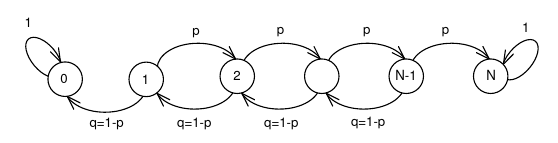
\includegraphics[scale=0.5]{images/ruine_joueur}
     \caption{Ruine du joueur sur $N$ états, à deux barrières absorbantes}
     \label{fig:ruine_joueur}
\end{figure}
Nous avons un graph à $N+1$ états, comme représenté à la Figure \ref{fig:ruine_joueur}. Nous commençons par imaginer que la probabilité $p = \frac{1}{2}$ (jeu pile/face). Nous calculons immédiatement, pour $\mathcal{A} = \{0\}$
\[h_{i0} = \left\{\begin{array}{ll}
    1 & i=0\\
    \\
    0 & i=N
\end{array}\right.\]
Pour calculer tous les cas intermédiaires, nous appliquons le théorème suivant :
\begin{boite}
    \evid{Théorème 5:} Le vecteur des probabilités $\mathbf{h}_\mathcal{A} = [h_{i\mathcal{A}},i \in \mathcal{A}]$ est la solution minimale non négative du système d'équations linéaire
    \begin{equation}
        \begin{array}{ll}
        h_{i\mathcal{A}} = 1 & \text{si } i \in \mathcal{A}\\
        h_{i\mathcal{A}} = \sum_{j \in \mathcal{S}}p_{ij}h_{j\mathcal{A}} & \text{si } i \notin \mathcal{A}
    \end{array}
\end{equation}
Démonstration : voir annexe {todo}
\end{boite}

Ainsi, pour tous les $1 \leq i \leq N-1$ nous avons 
\[h_{i0} = \sum_{j \in \mathcal{S}} p_{ij} h_{j0} = p\cdot h_{i+1,0} + q \cdot h_{i-1,0} \iff p\cdot h_{i+1,0} - h_{i,0} + q\cdot h_{i-1,0} = 0\]
En posant $\alpha,\beta$ les racines distinctes de $px^2 - x + q = 0$ nous avons
\[h_{i,0} = K_a \alpha^i + K_b \beta^i\]
Nous trouvons les racines :
\[\alpha,\beta = \frac{1\pm \sqrt{1-4(p(1-p)}}{2p} = \frac{1 \pm (1-2p)}{2p} = \left\{1,\frac{1-p}{p}\right\} = \left\{\alpha,\beta\right\}\]
Si $p \neq 1/2$. 

\todo{Rajouter conclusion}

\paragraph{Ruine du joueur sur \N}
Ici nous ne pouvons plus terminer à $N$, car notre adversaire a une fortune illimitée. 

\todo{rajouter ?}

Nous nous intéressons d'autre part au temps moyen que prend $X(n)$ pour atteindre le sous-ensemble $\mathcal{A}$ :
\[\mu_{i\mathcal{A}}^H = E[H_\mathcal{A} |X(0) = i] = \sum_{m \in \N \cup \{\infty\}} m P(H_\mathcal{A} = m | X(0) = i)\]
Que l'ont peut expliciter comme :
\begin{equation}
	\mu_{i\mathcal{A}}^H = \sum_{m \in \N} m P(X(m) \in \mathcal{A} \text{ et } X(n) \notin \mathcal{A} \text{ pour } 0 \leq n \leq m-1 | X(0) = i) 
\end{equation}
Ainsi, nous avons le théorème suivant :

\begin{boite}
	\evid{Théorème} Le vecteur des temps moyen d'atteinte $\boldsymbol{\mu}_\mathcal{A}^H = [\mu_{i\mathcal{A}}^H, i \in \mathcal{S}]$ est la solution minimale non négative du système d'équations linéaire
	\begin{equation}
            \begin{array}{ll}
                \mu_{i\mathcal{A}}^H = 0 & \text{si } i \in \mathcal{A}\\
                \mu_{i\mathcal{A}}^H = 1 + \sum_{j \notin \mathcal{A}}p_{ij}\mu_{j\mathcal{A}}^H & \text{si } i \notin \mathcal{A}
            \end{array}
	\end{equation}
\end{boite}

\subsubsection{Chaînes réversibles}
\paragraph{Définition}

Supposons une chaîne de Markov ergodique à l'état stationnaire, et qu'à partir d'un temps $n$ nous considérons la séquence d'états $X(n), X(n-1), X(n-2),...,X(0)$ c'est à dire la chaîne originelle en remontant le temps (\textbf{backward chain}). C'est également une chaîne de Markov car nous pouvons montrer que $P(X(n) = j | X(n+1) = i, X(n+1) = k,...) = P(X(n) = j | X(n+1) = i)$. De plus, en utilisant Bayes on peut calculer les probabilités de transitions de la chaîne ``renversée'' :
\begin{equation}
    \tilde{p}_{ij} = \frac{p_{ji}\pi_j^*}{\pi_i^*}
\end{equation}




%%%%%%%%%%%%%%%%%%%%%%%%%%%%%%%%%%%%%%%%%%%%%%
%%%%%%%%%%%%%%%    MODULE 7     %%%%%%%%%%%%%%
%%%%%%%%%%%%%%%%%%%%%%%%%%%%%%%%%%%%%%%%%%%%%%
\section{Chaînes de Markov à temps continu}
\subsection{Introduction}
\subsubsection{Première définition}
Nous considérons maintenant des temps continu, c'est à dire $\{x(t), t \in \R^+\}$. Cet ensemble est une chaîne de Markov si, $\forall t_0 < t_1 < t_2 < ... t_n \in \R^+\ \forall i_0,i_1,...,i_n \in \mathcal{S}_X$ nous avons
\begin{equation}
    P(X(t_n) = i_n | X(t_{n-1}) = i_{n-1},...,X(t_0) = i_0) = P(X(t_n) = i_n | X(t_{n-1}) = t_{n-1})
\end{equation}
et que le processus est homogène pour tout $s,t \in \R^+$ et $i,j \in \mathcal{S}$
\[P(X(t+s) = j | X(s) = i) = p_{ij}(t) = P(X(t) = j | X(0) = i)\]
Les probabilités $p_{ij}(t)$ sont posées dans une matrice de transition $P(t)$, et les probabilités d'état $\pi_i(t) = P(X(t) = i)$ sont posées dans le vecteur d'état $\boldsymbol{\pi}(t) = [ \pi_0(t)\ \pi_1(t)\ \pi_2(t)\ \cdots\ ]$.

A cette chaine sont associés des processus stochastiques, comme pour les processus de comptage, Tout d'abord la \textit{séquence des temps de transition} (jump times) $\{S(n), n \in \N\}$ avec $0 ) S(0) < S(1) < ... < S(n) < S(n+1) < ...$ où $S(n)$ est \uline{le temps où se produit la $n$ième transition d'un état à l'autre}. Ensuite la \textit{séquence des temps de séjour} (holding times)  $\{T(n), n \in \N\}$ qui décrit \uline{l'intervalle de temps pendant lequel le processus reste dans un même état} (donc temps entre deux transitions successives). Les trois processus $X, S, T$ sont liés :
\todo{liaison}

\subsubsection{Distribution des temps de séjour}
Nous montrons facilement, en utilisant les propriétés d'un processus Markovien, que les temps de séjour sont une suite de variables aléatoires indépendantes (pas identiquement distribuées), avec une distribution exponentielle $exp(\nu_i)$, avec
\[\nu_i = \frac{1}{E[T_i(n)]}\]
Soit l'inverse de la durée moyenne pendant laquelle le processus va séjourner en $i$.

\subsubsection{Chaînes de Markov induites}
Maintenant que nous avons le temps moyen que nous restons à chaque état, reste à déterminer la probabilité d'atteindre un autre état. En effet, chaque fois que la chaîne quitte l'état $i$, elle doit entrer en état $j \in \mathcal{S}$ avec une probabilité de $\hat{q}_{ij}$ qui vérifie trivialement
\begin{equation}
    \hat{q}_{ii} = 0 \qquad \sum_{j \in \mathcal{S}} \hat{q}_{ij} = 1
\end{equation}

A partir de $\{X(t), t \in \R^+\}$ on construit le processus à temps discret $n \in \N$ :
\begin{equation}
    \hat{X}(n) = X(S(n))
\end{equation}
qui est donc la séquence des différentes valeurs prises par $X(t)$. C'est clairement une chaîne de Markov à temps discret dont les probabilités de transition $i\to j$ sont les $\hat{q}_{ij} = P(\hat{X}(n) = j | \hat{X}(n-1) = i)$

\subsubsection{Équations de Kolmogorov}
Dans le cas continu, les équations de Chapman-Kolmogorov s'écrivent
\begin{equation}
    p_{ij}(t_1 + t_2) = \sum_{k \in \mathcal{S}}p_{ik}(t_1)p_{kj}(t_2)
\end{equation}
Nous définissons aussi les probabilités d'état :
\[\begin{array}{l}
    \pi_i(t) = P(X(t) = i)\\
    \pi_i(t+s) = \somme{}{k\in \mathcal{S}} \underbrace{P(X(t+s) = i |X(t) = k)}_{p_{ki}(s)} \underbrace{P(X(t) = k)}_{\pi_k(t)} = \somme{}{k \in \mathcal{S}} \pi_l(t) p_{ki}(s)
\end{array}\]

\todo{Transition}

\begin{equation}
    Q = [q_{ij}]_{i,j \in \mathcal{S}_X}
\end{equation}

Pour une chaîne à temps discret, si elle est irréductible ($i \leftrightarrow j \forall i,j \in \mathcal{S}_X$), apériodique et récurrente positive, alors 
\[\exists ! \boldsymbol{\pi}^* \text{ telle que } \boldsymbol{\pi} = \boldsymbol{\pi}P \text{ et } \limite{\ninf} \boldsymbol{\pi}(n) = \boldsymbol{\pi}^*\]
Pour le temps continu, il suffit de vérifier si la chaîne induite est irréductible et récurrente positive.








%%%%%%%%%%%%%%%%%%%%%%%%%%%%%%%%%%%%%%%%%%%%%%
%%%%%%%%%%%%%%%    Module 8     %%%%%%%%%%%%%%
%%%%%%%%%%%%%%%%%%%%%%%%%%%%%%%%%%%%%%%%%%%%%%

\section{Files d'attente}

%%%%%%%%%%%%%%%%%%%%%%%%%%%%%%%%%%%%%%%%%%%%%%
%%%%%%%%%%%%%%%    APPENDIX     %%%%%%%%%%%%%%
%%%%%%%%%%%%%%%%%%%%%%%%%%%%%%%%%%%%%%%%%%%%%%
\appendix
\titleformat{\section}{\large\bfseries}{}{0pt}{\thesection\quad}
\numberwithin{equation}{subsection}
\section{Preuves}
\subsection{Chapitre 1}
\subsubsection{Fonction d'une variable aléatoire}
\label{preuve_fonction_va}
Comme nous avons $Y = g(x)$, alors on peut prendre un $y$, une valeur particulière de $Y$, et de ceci en découlent $x_1,x_2,\ldots,x_m$ les $m$ racines respectives de l'équation $y = g(x_i)$ avec $1 \leq i \leq m$.

Nous voulons poser $A$ l'événement 
\[A = \{\zeta| y < Y(\zeta) \leq y+\Delta y\}\]
Nous choisissons une espace de plus d'une valeur, car comme démontré plus haut la probabilité $P(Y=y)$ est nulle. Nous savons par les propriétés établies plus tôt que la probabilité que cet événement se produise est 
\begin{equation}
    P(A) = P(y \leq Y \leq y+\Delta y) = f_Y(y)|\Delta y|
    \label{eq_fonction_va_1}
\end{equation}
si $\Delta y \to 0$. De plus, comme $Y(\zeta) = g(X(\zeta))$ et que $g(x)$ est continue, nous pouvons réécrire $A$ comme
\[\begin{array}{lll}
    A   &=& \{\zeta | y <  g(X(\zeta)) \leq y+\Delta y\}\\
        &=& \{\zeta | x_1 < X(\zeta) \leq x_1+\Delta x_1\} \cup \\
        &&\{\zeta | x_2 < X(\zeta) \leq x_2+\Delta x_2\} \cup \cdots \cup\\
        && \{\zeta | x_m < X(\zeta) \leq x_m+\Delta x_m\}
\end{array}\]
Ce qui nous permet d'écrire :
\begin{equation}
    P(A) = f_X(x_1)|\Delta x_1)| + f_X(x_2)|\Delta x_2| + \ldots
    \label{equ_fonction_va_2}
\end{equation}
En se rappelant que $g'(x_i) = \limite{\Delta x_i \to 0} \frac{\Delta y}{\Delta x_i}$ et en égalant (\ref{eq_fonction_va_1}) et (\ref{equ_fonction_va_2}), nous trouvons 

\begin{equation}
    f_Y(y) = \somme{}{i}\frac{f_X(x_i)}{|g'(x_i)}
\end{equation}
\subsubsection{Existence de la fonction caractéristique}
\label{preuve_existence_fonc_carac}
\[\Phi_X(\omega) \leq |\Phi_X(\omega)| = \left|\infint e^{j\omega x} f_X(x)\deriv{x}\right| \leq \infint \left|e^{j\omega x}f_X(x)\right|\deriv{x} = \infint f_X(x)\deriv{x} = 1\]

\subsubsection{Moment d'ordre k avec la fonction caractéristique}
\label{preuve_momentK_foncCarac}
Nous dérivons $\Phi_X(\omega)$ par rapport à $\omega$ et l'évaluons en $\omega = 0$ (maximum de la fonction caractéristique) :
\begin{equation}
    \left.\frac{\deriv{\Phi_X(\omega)}}{\deriv \omega}\right|_{\omega = 0} = \left.\infint jxe^{j\omega x}f_X(x)\deriv{x}\right|_{\omega = 0} = j\infint xf_X(x) \deriv{x} = jE[X]
\end{equation}
Ce qui donne 
\begin{equation}
    E[X] = \frac{1}{j} \left.\frac{\deriv{\Phi_X(\omega)}}{\deriv \omega}\right|_{\omega = 0}
\end{equation}
Et en répétant l'opération, nous voyons rapidement que 
\begin{equation}
    E[X^k] = \frac{1}{j^k} \left.\frac{\deriv^k\Phi_X(\omega)}{\deriv \omega^k}\right|_{\omega = 0}
\end{equation}
\subsubsection{Inégalité de Markov}
\label{preuve_inegalite_markov}
Lorsque la v.a. $X$ ne prend pas de valeurs négatives, et ne limitant $a > 0$, on observe :
\begin{equation}
    \begin{array}{ll}
        E[X]     &= \infint xf_X(x) \deriv{x} = \int_0^a xf_X(x) \deriv{x} + \int_a^\infty xf_X(x) \deriv{x}\\
                 &\geq \int_a^\infty xf_X(x) \deriv{x} \geq  \int_a^\infty af_X(x) \deriv{x} = a\int_a^\infty f_X(x) \deriv{x} = aP(X \geq a)
    \end{array}
\end{equation}
Ce qui implique que e
\begin{equation}
    P(X \geq a) \leq \frac{E[X]}{a}
\end{equation}
Toujours en conservant les conditions $X \geq 0$, $a > 0$.
\subsubsection{Inégalité de Chebychev}
\label{preuve_inegalite_chebychev}
En considérant la v.a. $D = (X-\mu_X)^2$, dont la moyenne est $E[D] = E[(X-\mu_X)^2] = \sigma_X^2$ (c'est à dire la variance de $X$. Posons $b = \sqrt{a}$ dans l'inégalité de Markov (voir \ref{preuve_inegalite_markov}) :
\[P(D \geq b^2) \leq \frac{\sigma_X^2}{b^2}\]
Or, comme $P(D \geq b^2) = P((X-\mu_x)^2 \geq b^2) = P(|X-\mu_x| \geq b)$ nous avons
\begin{equation}
    P(|X-\mu_X| \geq b) \leq \frac{\sigma_X^2}{b^2}
\end{equation}

\subsubsection{Limite d'une v.a. binomiale vers Poisson}
\label{preuve_limite_binomiale_poisson}
Partons avec $k=0$ ; comme $\binom{n}{0} = 1$, on a 
\[p_0 = (1-p)^n \overset{\mu=np}{\longeq} (1-\mu/n)^n \overset{\ninf}{\longrightarrow} e^{-\mu}\]
Pour $k > 0$ :
\[\frac{p_{k+1}}{p_k} = \frac{\binom{n}{k+1}p^{k+1}(1-p)^{n-k-1}}{\binom{n}{k}p^k(1-p)^{n-k}} = ... = \frac{\mu(1-k/n)}{(k+1)(1-\mu/n)} \overset{\ninf}{\longrightarrow} \frac{\mu}{k+1}\]
Ce qui donne la limite
\[p_{k+1} \to \frac{\mu}{k+1}p_k \to \frac{\mu}{k++}\frac{\mu}{k}p_{k-1} \to ... \to \frac{\mu^{k+1}}{(k+1)!}e^{-\mu}\]

\subsection{Chapitre 2}
\subsubsection{La somme de deux v.a. indépendantes est le produit de convolution}
\label{preuve_somme_va_produit_convo}
\todo{definitely todo}
\subsection{Chapitre 3}
\subsection{Chapitre 4}
\subsection{Chapitre 5}
\subsubsection{Les deux définitions du processus de Poisson homogène sont équivalentes}
\label{preuve_egalite_definitions_processus_poisson}    
\end{document}